%\documentclass[10pt,oneside,a4paper,openany,draft]{article}
\documentclass[10pt,a4paper,openany]{article}

%%%%%%%%%%%%%%%%%%%%%%%%%%%%%%%%%%%%%%%%%%%%%%%%%%%%%%%%%%%%%%%%%%%%%%%%%%%%%%%
%---Preamble---
%%%%%%%%%%%%%%%%%%%%%%%%%%%%%%%%%%%%%%%%%%%%%%%%%%%%%%%%%%%%%%%%%%%%%%%%%%%%%%%
\usepackage{amssymb,amsmath}
\usepackage{array}
\usepackage{authblk}
\usepackage{microtype}
\usepackage[font={small}]{caption}
\usepackage{booktabs}
\usepackage{textcomp}
\usepackage{color}
\usepackage{lineno}
\usepackage[nottoc]{tocbibind}
\usepackage{graphicx}
\usepackage{hyperref}
\usepackage[margin=1in,bindingoffset=.2in]{geometry}
\usepackage{caption}
\usepackage{subcaption}
\usepackage{rotating}
\usepackage{lscape}
\usepackage{pdfpages}
\usepackage{physics}
\usepackage[compat=1.1.0]{tikz-feynman}
\usepackage[labelfont=bf]{caption}

\graphicspath{{plots/2x2/}}
\renewcommand{\refname}{References}
\setcounter{MaxMatrixCols}{10}


%%%%%%%%%%%%%%%%%%%%%%%%%%%%%%%%%%%%%%%%%%%%%%%%%%%%%%%%%%%%%%%%%%%%%%%%%%%%%%%
%---Document---
%%%%%%%%%%%%%%%%%%%%%%%%%%%%%%%%%%%%%%%%%%%%%%%%%%%%%%%%%%%%%%%%%%%%%%%%%%%%%%%
\begin{document}
\linenumbers

%%%%%%%%%%%%%%%%%%%%%%%%%%%%%%%%%%%%%%%%%%%%%%%%%%%%%%%%%%%%%%%%%%%%%%%%%%%%%%%
%---Title---
%%%%%%%%%%%%%%%%%%%%%%%%%%%%%%%%%%%%%%%%%%%%%%%%%%%%%%%%%%%%%%%%%%%%%%%%%%%%%%%
\title{\Large \textbf{ArgonCube 2x2 Physics Study}}
\author[1]{P.~P.~Koller\thanks{Corresponding author: patrick.koller@lhep.unibe.ch}}
%\author[2]{\textit{et al.}}
\affil[1]{\textit{University of Bern, Albert Einstein Center for Fundamental Physics,
Laboratory for High Energy Physics (LHEP), Bern, Switzerland}}
%\affil[2]{\textit{Middle-earth}}
\date{\today}
\maketitle

%%%%%%%%%%%%%%%%%%%%%%%%%%%%%%%%%%%%%%%%%%%%%%%%%%%%%%%%%%%%%%%%%%%%%%%%%%%%%%%
%---Introduction Chapter---
%%%%%%%%%%%%%%%%%%%%%%%%%%%%%%%%%%%%%%%%%%%%%%%%%%%%%%%%%%%%%%%%%%%%%%%%%%%%%%%

\setcounter{secnumdepth}{2}		% section numbering depth
%\chapter*{}
%\addcontentsline{toc}{chapter}{Introduction}
\pagenumbering{arabic}

\subsection{Introduction}
\subsubsection{EM~Showers}
\begin{figure}[htbp]
	\centering
	\begin{subfigure}[b]{0.49\textwidth}
		\centering
		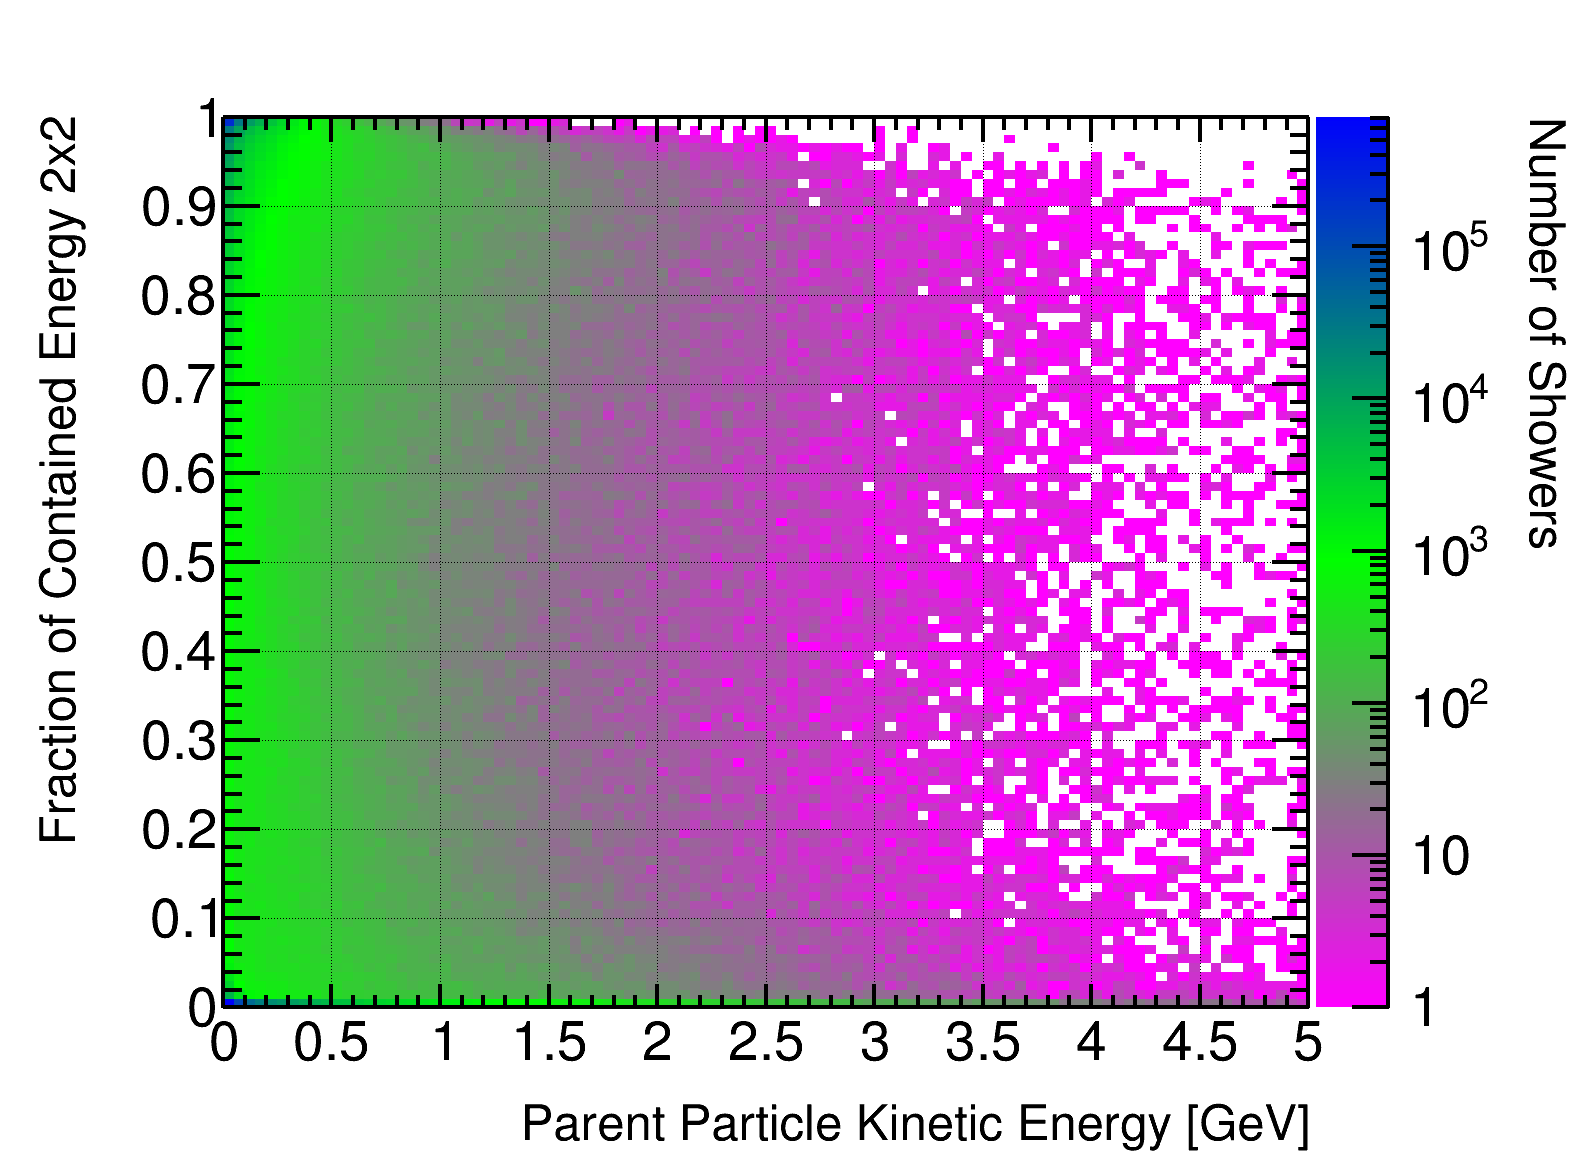
\includegraphics[width=1.0\textwidth]{EM_contained_frac_2x2.png}
		\caption{2x2 stand-alone, no fiducialisation.}
		\label{}
	\end{subfigure}	
	\hfill
	\begin{subfigure}[b]{0.49\textwidth}
		\centering
    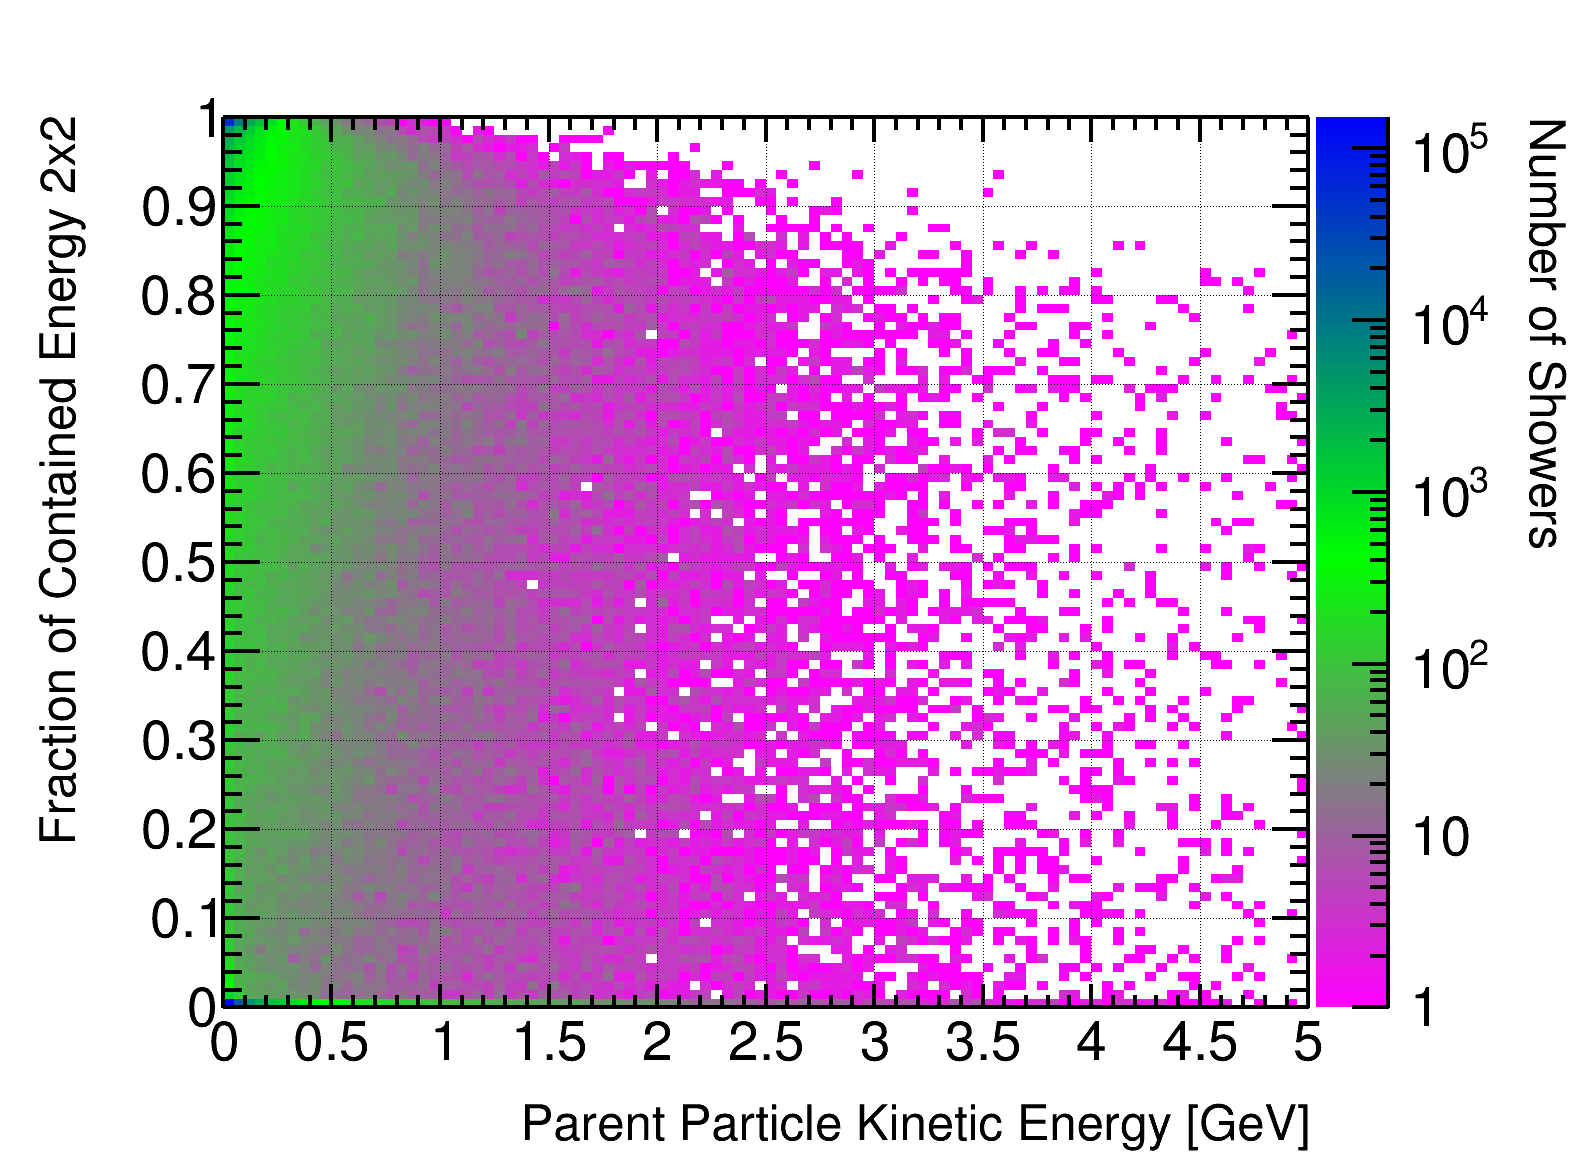
\includegraphics[width=1.0\textwidth]{EM_contained_frac_2x2_fiducial.png}
		\caption{2x2 stand-alone, vertex in fiducial volume.}
		\label{}
	\end{subfigure}	
	\begin{subfigure}[b]{0.49\textwidth}
		\centering
		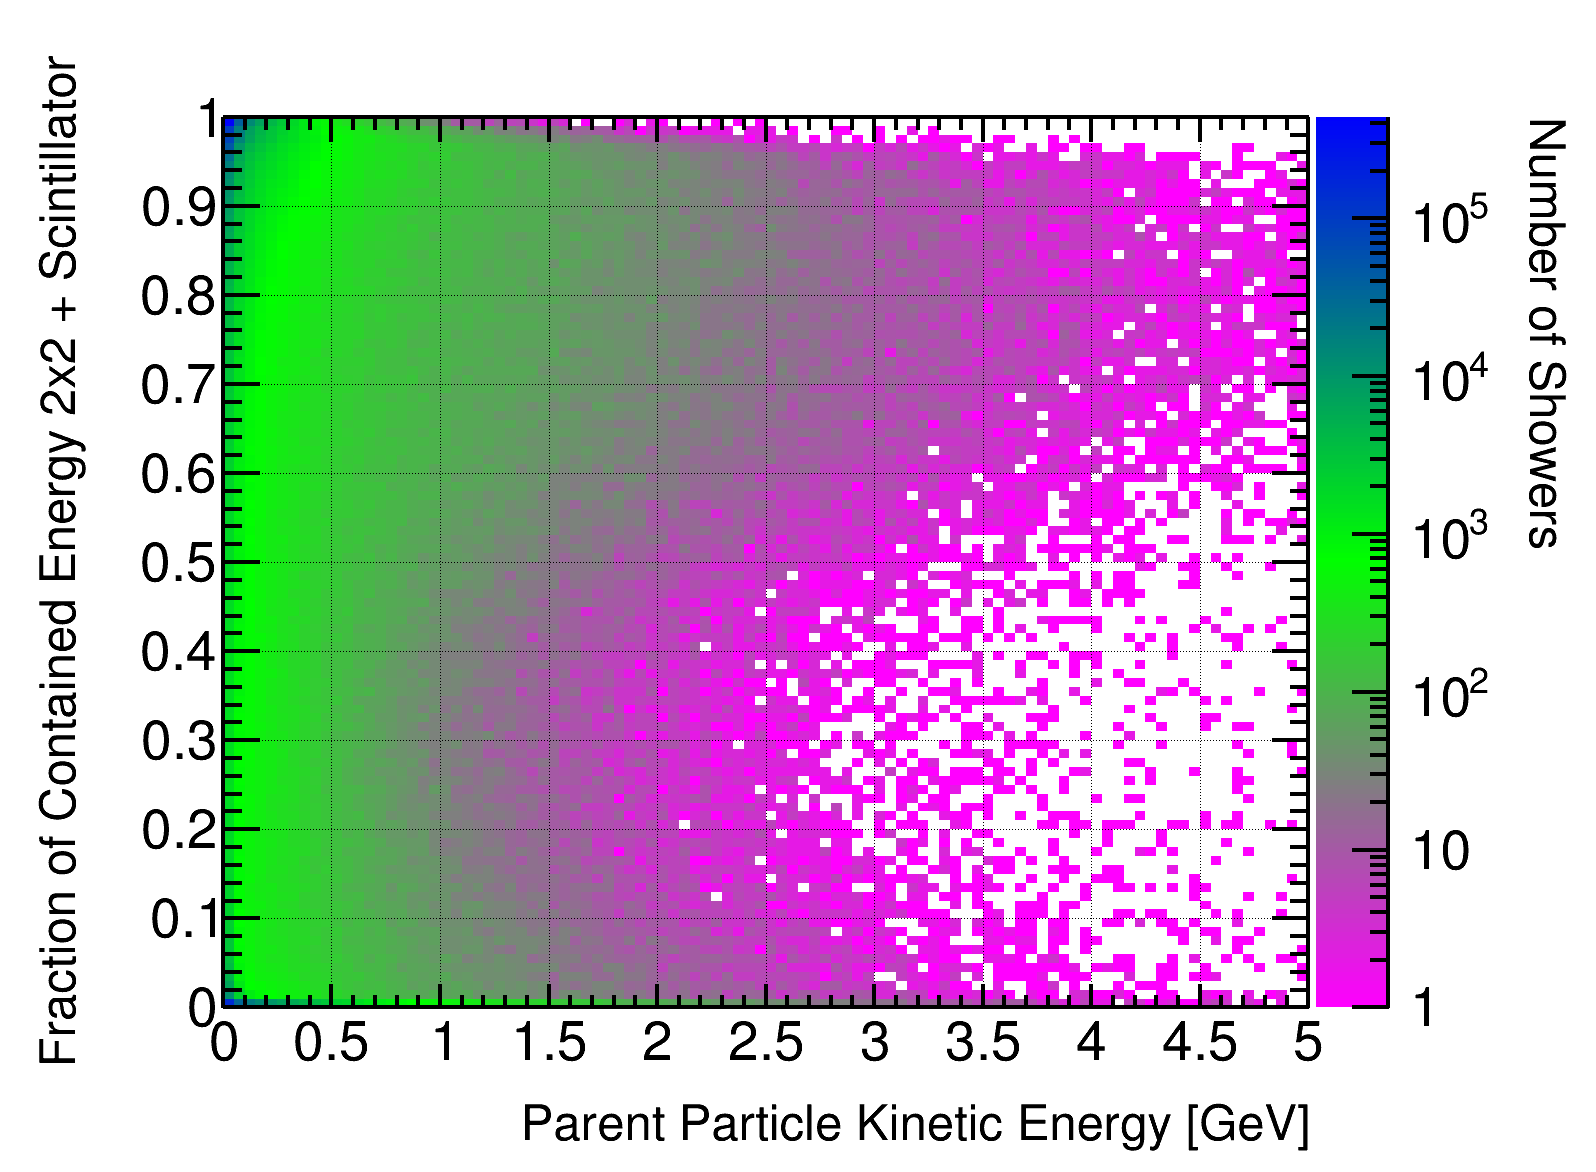
\includegraphics[width=1.0\textwidth]{EM_contained_frac_2x2_Scintillator_gap.png}
		\caption{2x2 + tracker, no fiducialisation.}
		\label{}
	\end{subfigure}	
	\hfill
	\begin{subfigure}[b]{0.49\textwidth}
		\centering
		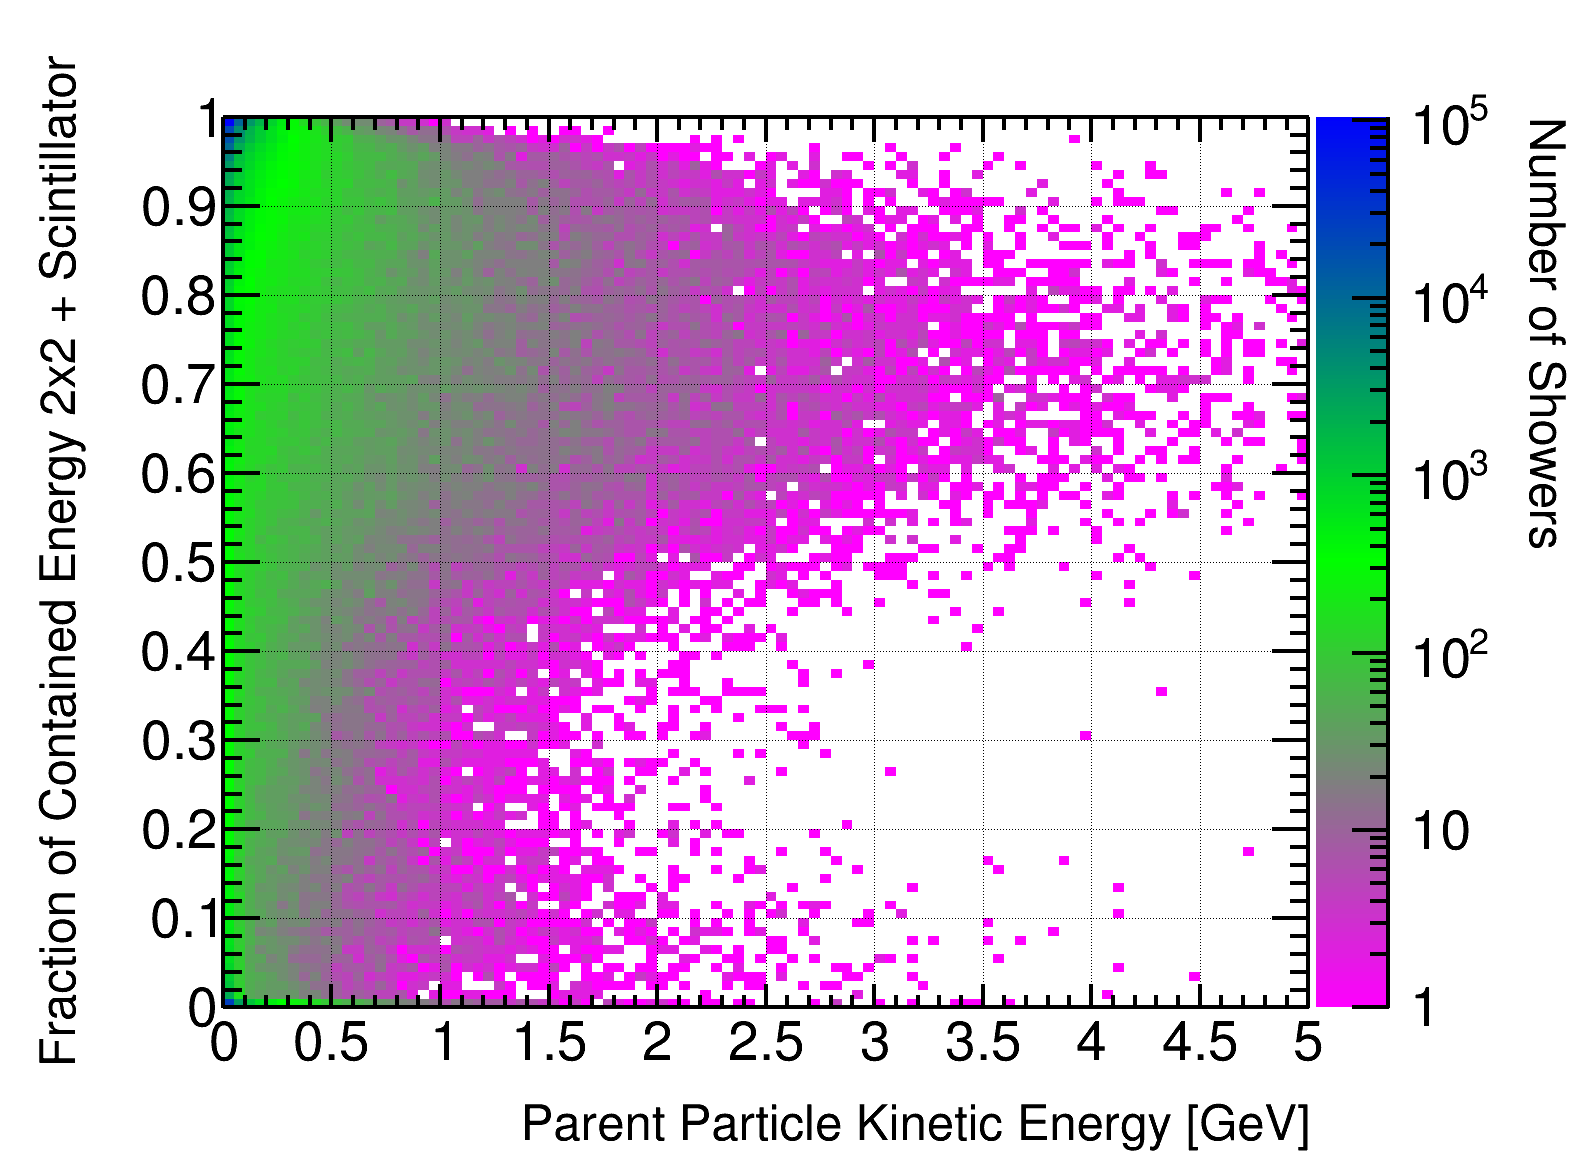
\includegraphics[width=1.0\textwidth]{EM_contained_frac_2x2_Scintillator_fiducial_gap.png}
		\caption{2x2 + tracker, vertex in fiducial volume.}
		\label{}
	\end{subfigure}
	\begin{subfigure}[b]{0.49\textwidth}
		\centering
		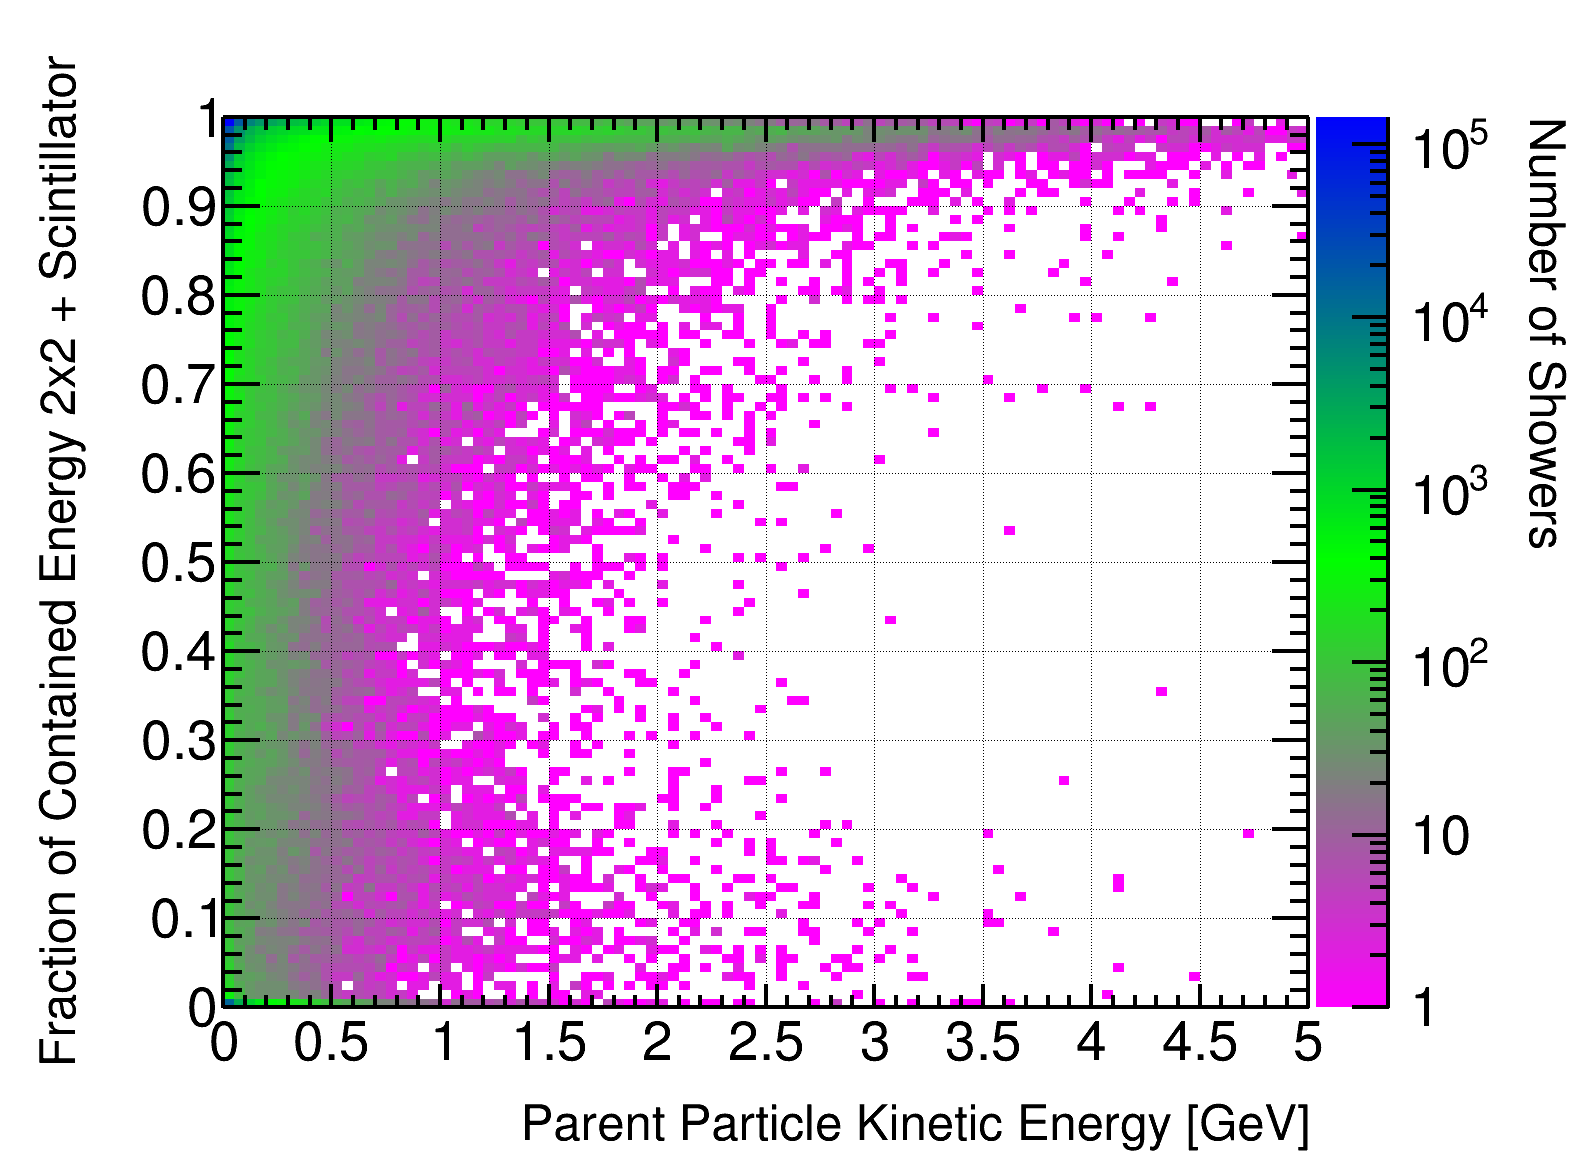
\includegraphics[width=1.0\textwidth]{EM_contained_frac_2x2_Scintillator_fiducial.png}
		\caption{2x2 + tracker no gap, vertex in fiducial volume.}
		\label{}
	\end{subfigure}	
  \caption{Fraction of kinetic shower energy ($e^{\pm}$~mass ignored) deposited within the active detector volume.}
\end{figure}

\begin{figure}[htbp]
	\centering
	\begin{subfigure}[b]{0.49\textwidth}
		\centering
		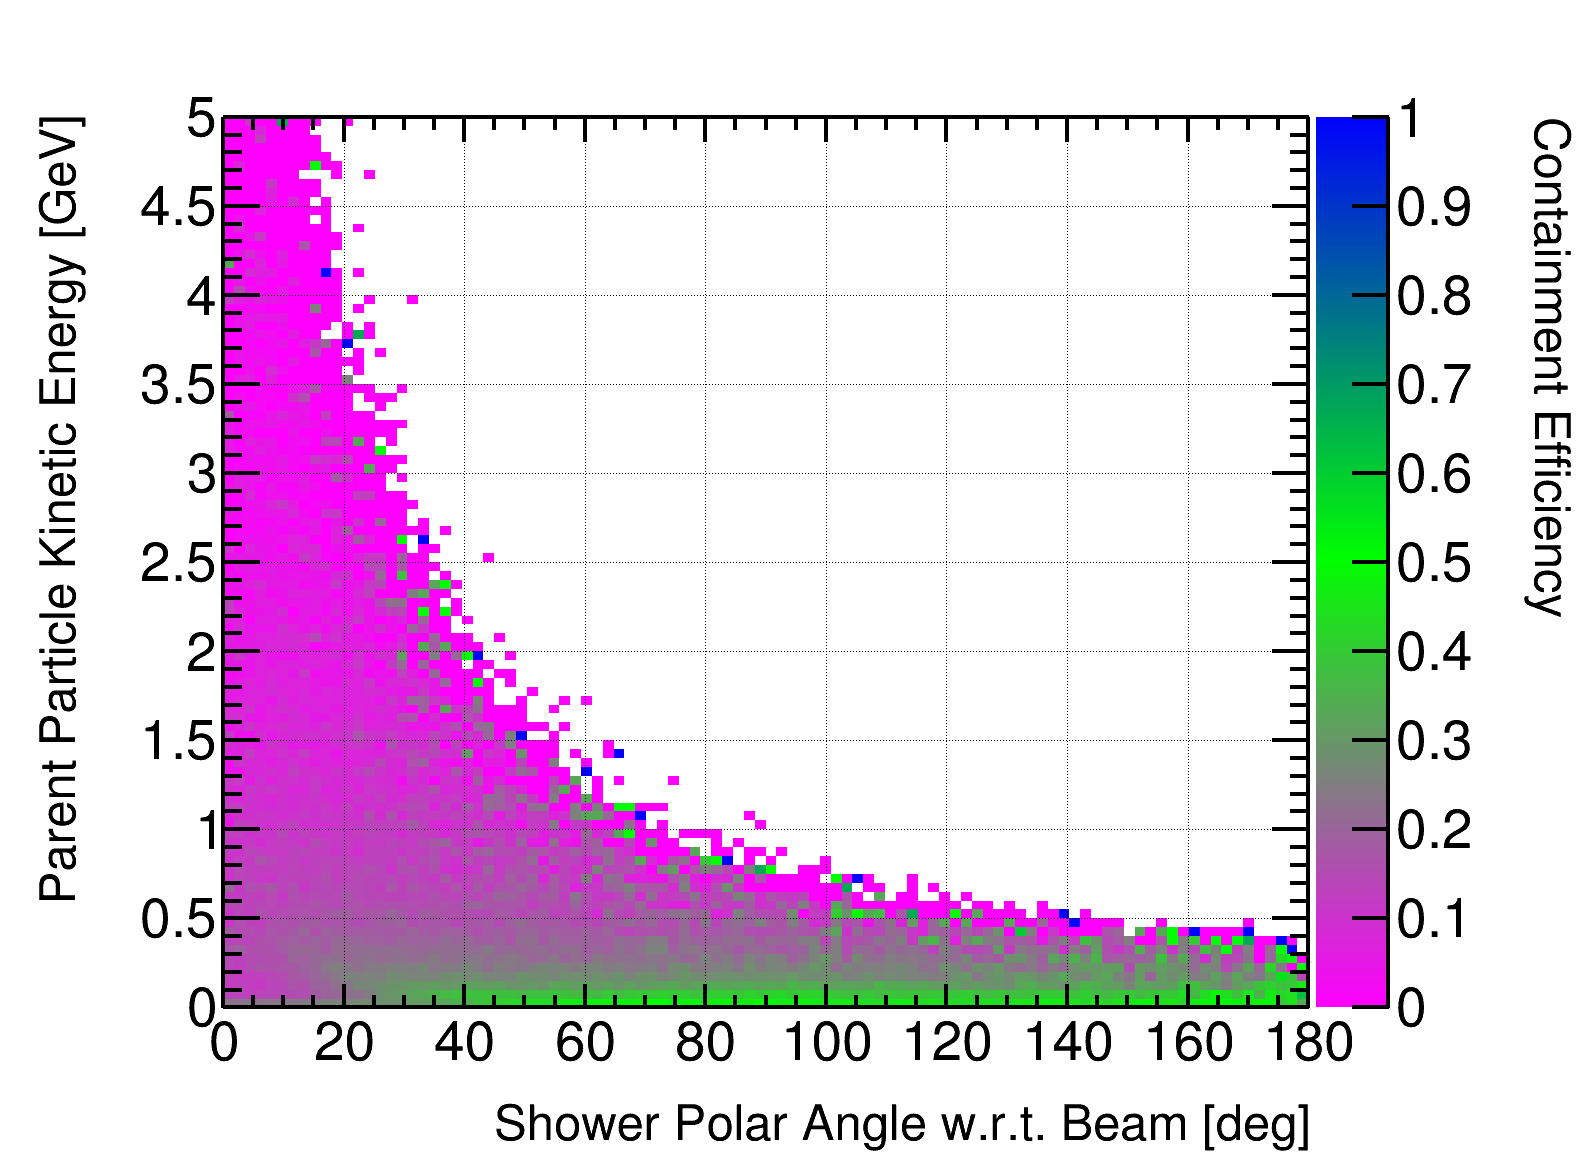
\includegraphics[width=1.0\textwidth]{EM_cont_eff_2x2.png}
		\caption{2x2 stand-alone, no fiducialisation.}
		\label{}
	\end{subfigure}	
	\hfill
	\begin{subfigure}[b]{0.49\textwidth}
		\centering
    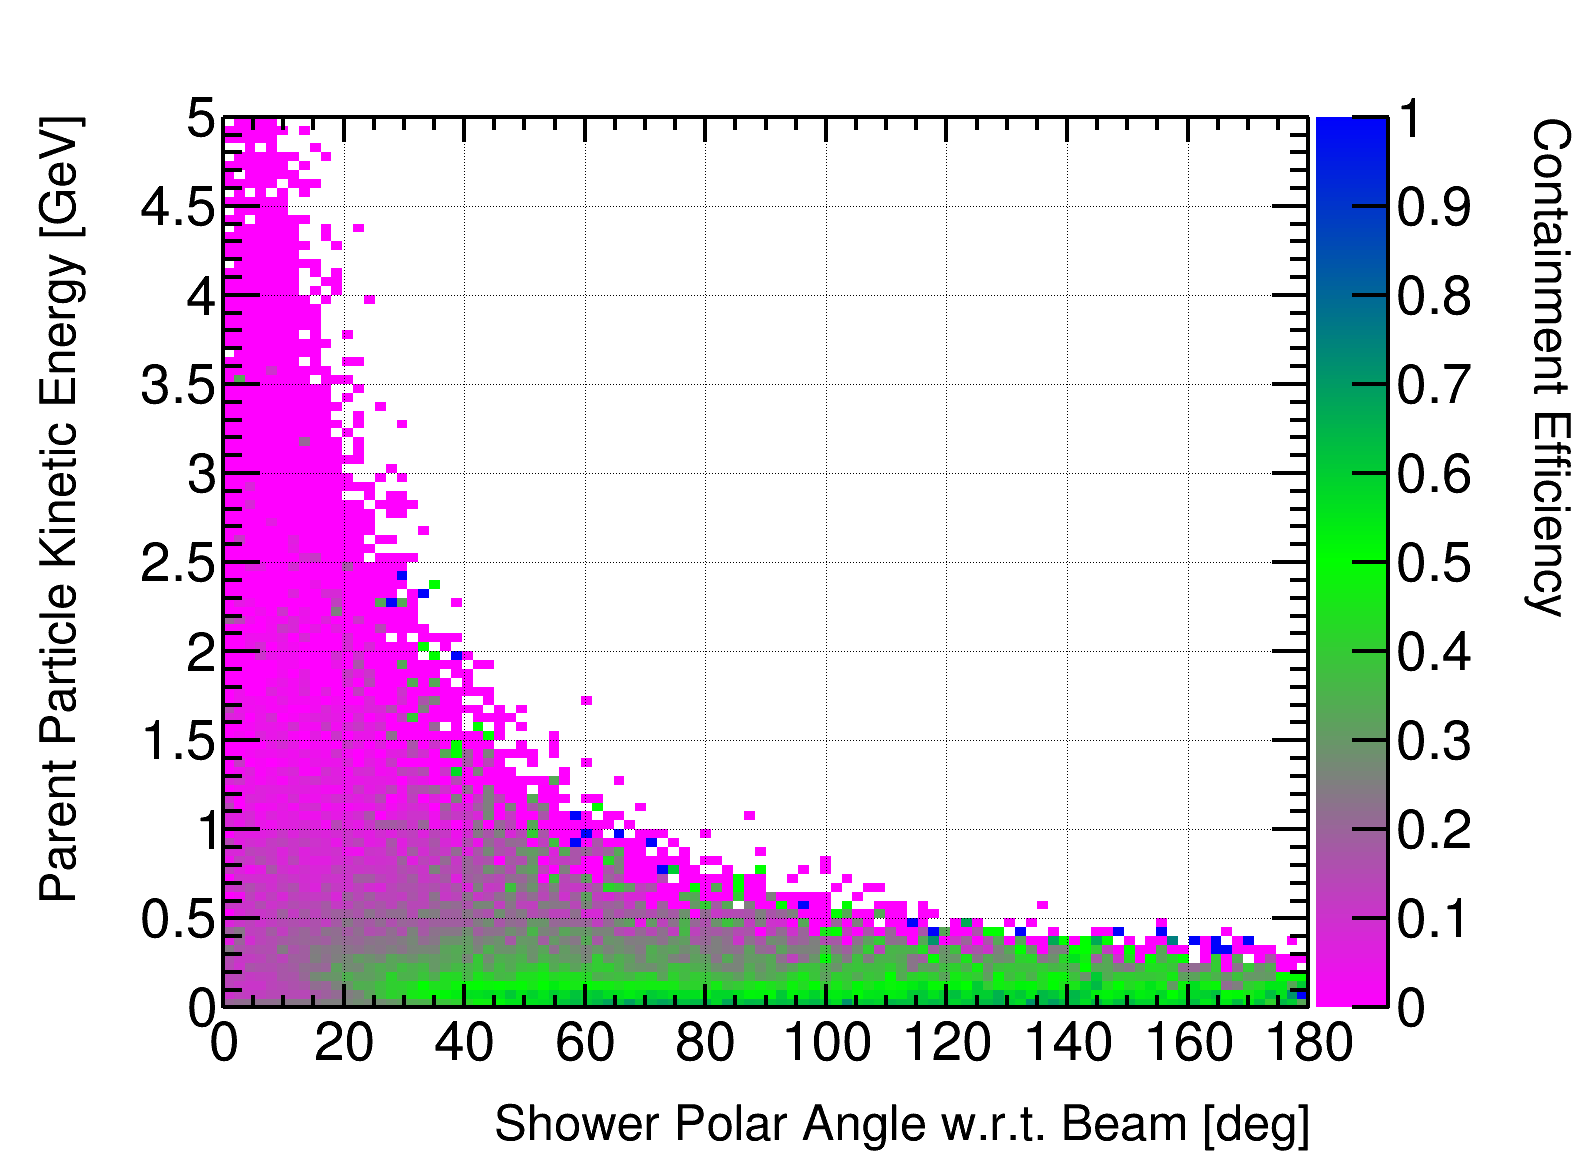
\includegraphics[width=1.0\textwidth]{EM_cont_eff_2x2_fiducial.png}
		\caption{2x2 stand-alone, vertex in fiducial volume.}
		\label{}
	\end{subfigure}	
	\begin{subfigure}[b]{0.49\textwidth}
		\centering
		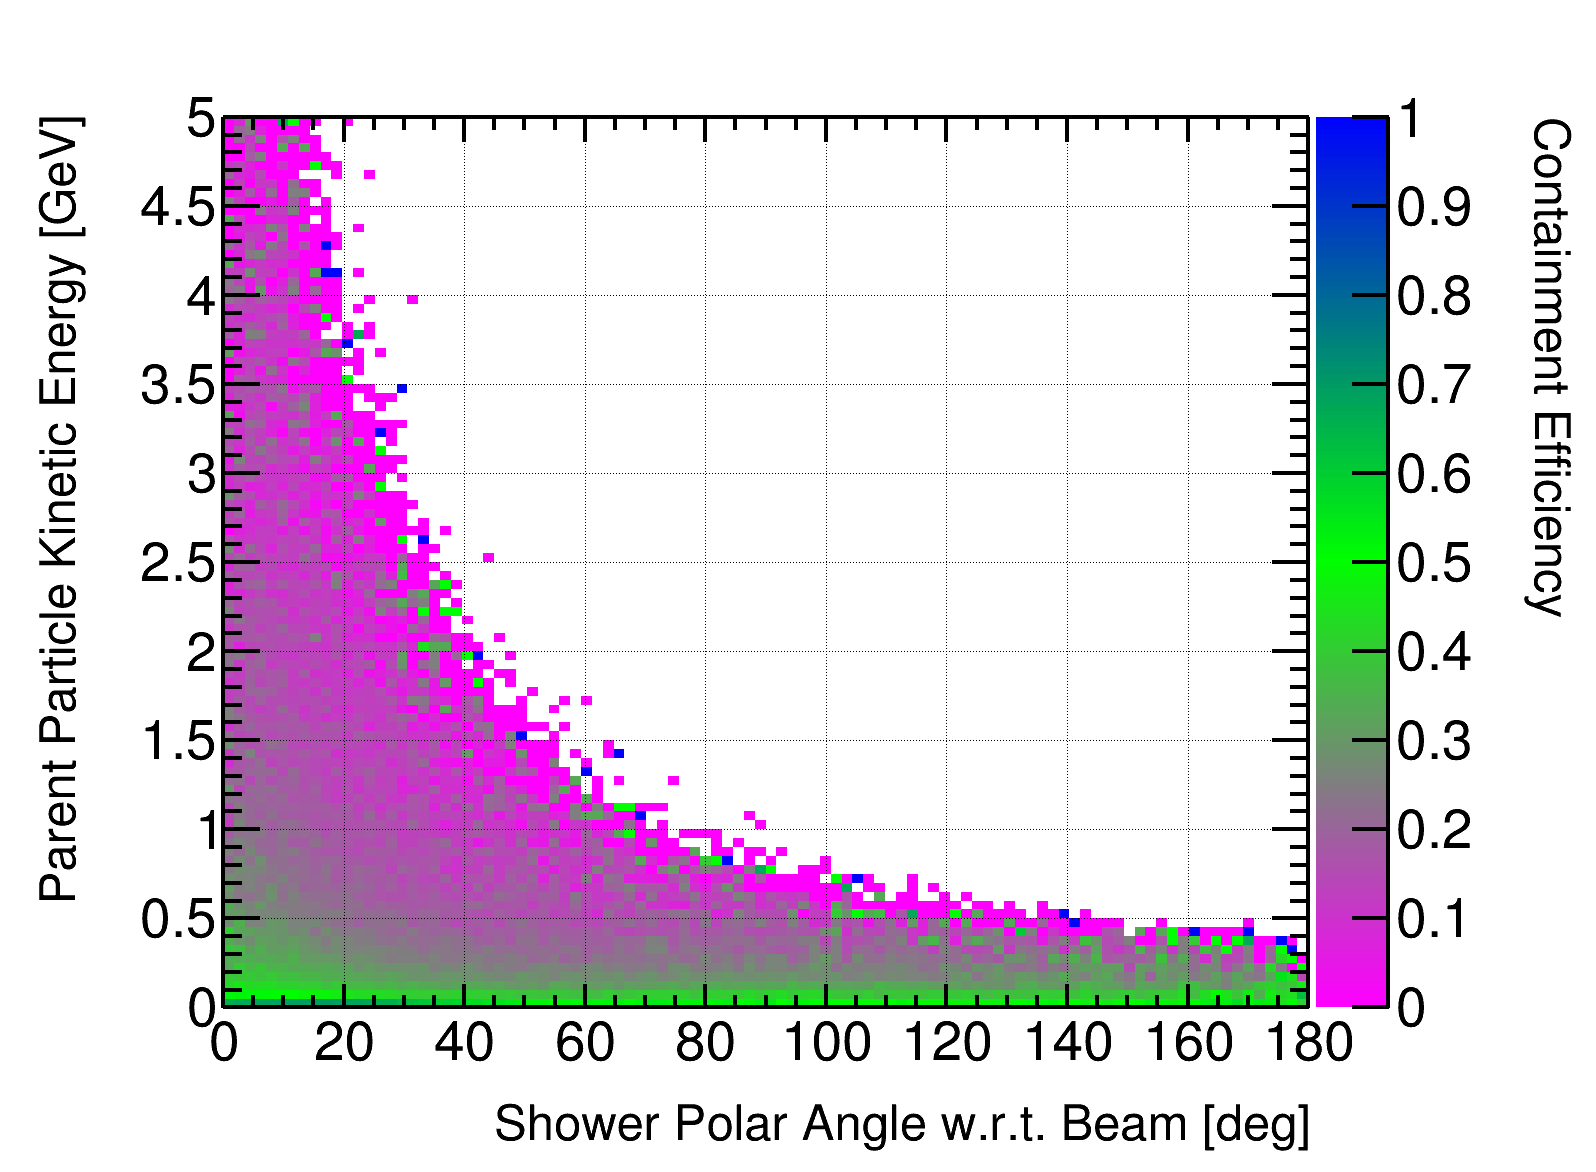
\includegraphics[width=1.0\textwidth]{EM_cont_eff_2x2_Scintillator_gap.png}
		\caption{2x2 + tracker, no fiducialisation.}
		\label{}
	\end{subfigure}	
	\hfill
	\begin{subfigure}[b]{0.49\textwidth}
		\centering
		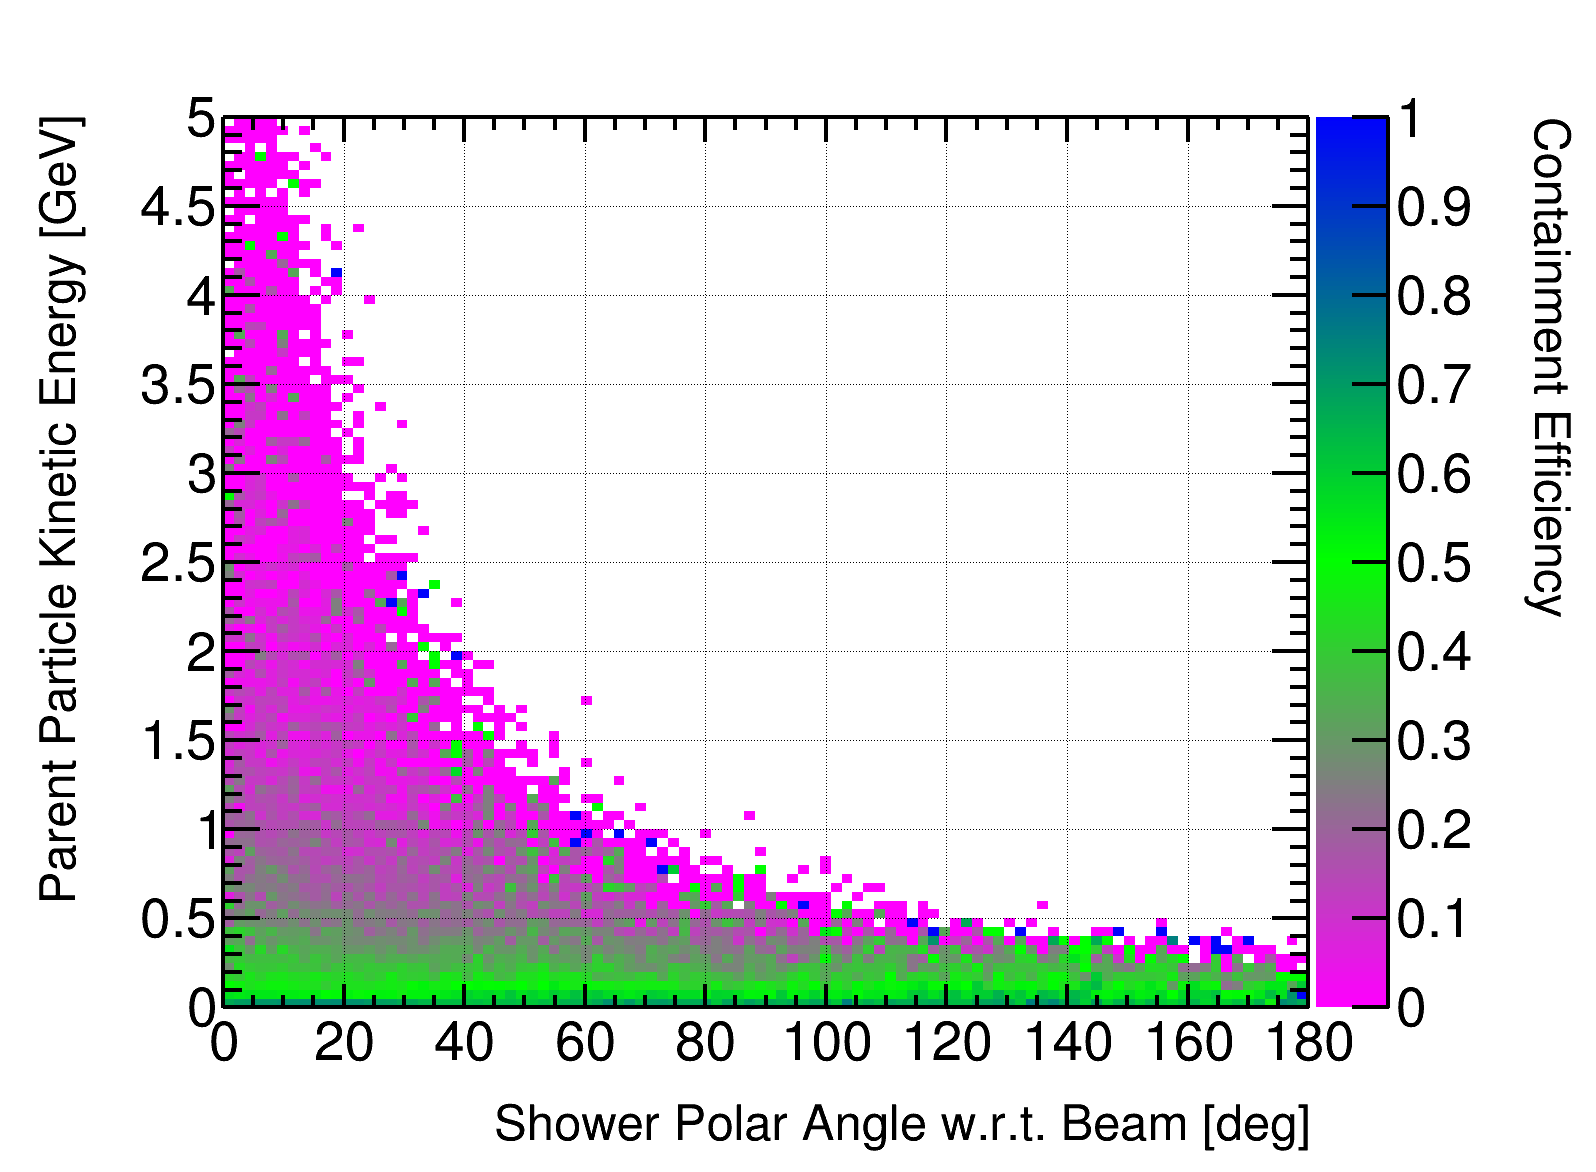
\includegraphics[width=1.0\textwidth]{EM_cont_eff_2x2_Scintillator_fiducial_gap.png}
		\caption{2x2 + tracker, vertex in fiducial volume.}
		\label{}
	\end{subfigure}
	\begin{subfigure}[b]{0.49\textwidth}
		\centering
		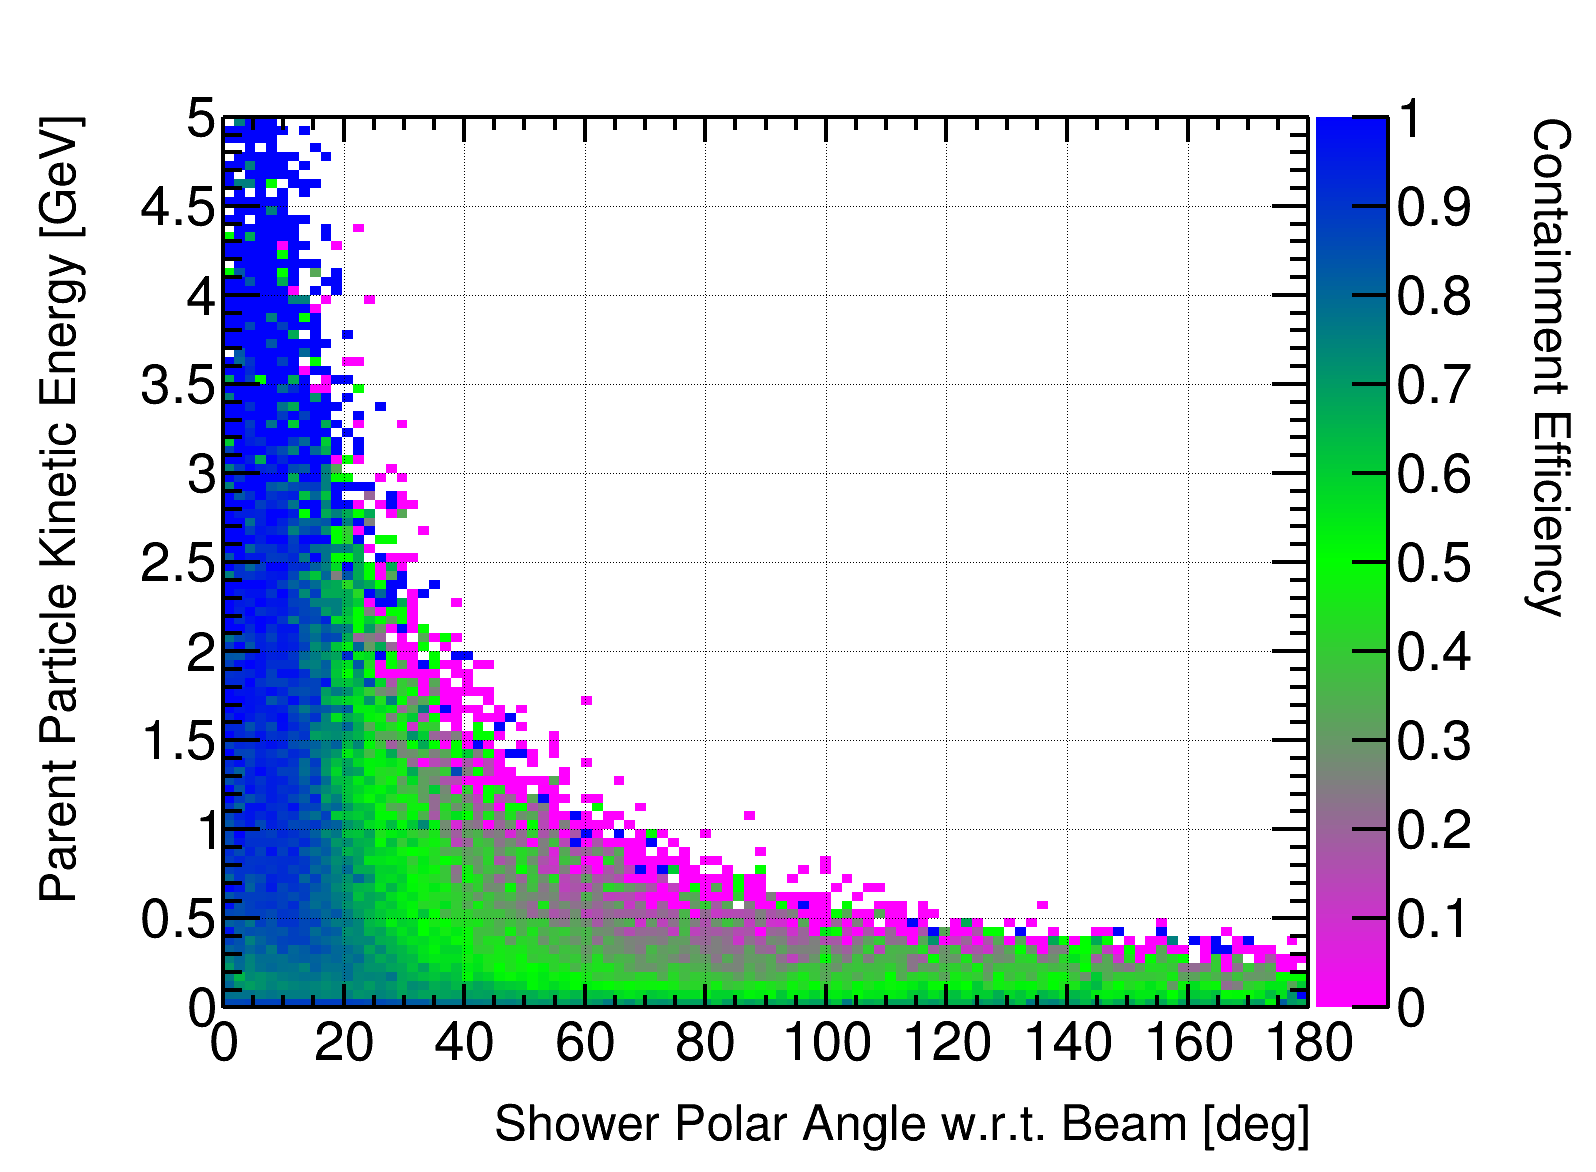
\includegraphics[width=1.0\textwidth]{EM_cont_eff_2x2_Scintillator_fiducial.png}
		\caption{2x2 + tracker no gap, vertex in fiducial volume.}
		\label{}
	\end{subfigure}	
	\caption{Shower-containment efficiency. A shower is classed as contained if at least 90\% of the kinetic shower energy ($e^{\pm}$~mass ignored) is deposited within the active detector volume.}
\end{figure}

\subsubsection{$\pi^{0}$~Showers}
\begin{figure}[htbp]
	\centering
	\begin{subfigure}[b]{0.49\textwidth}
		\centering
		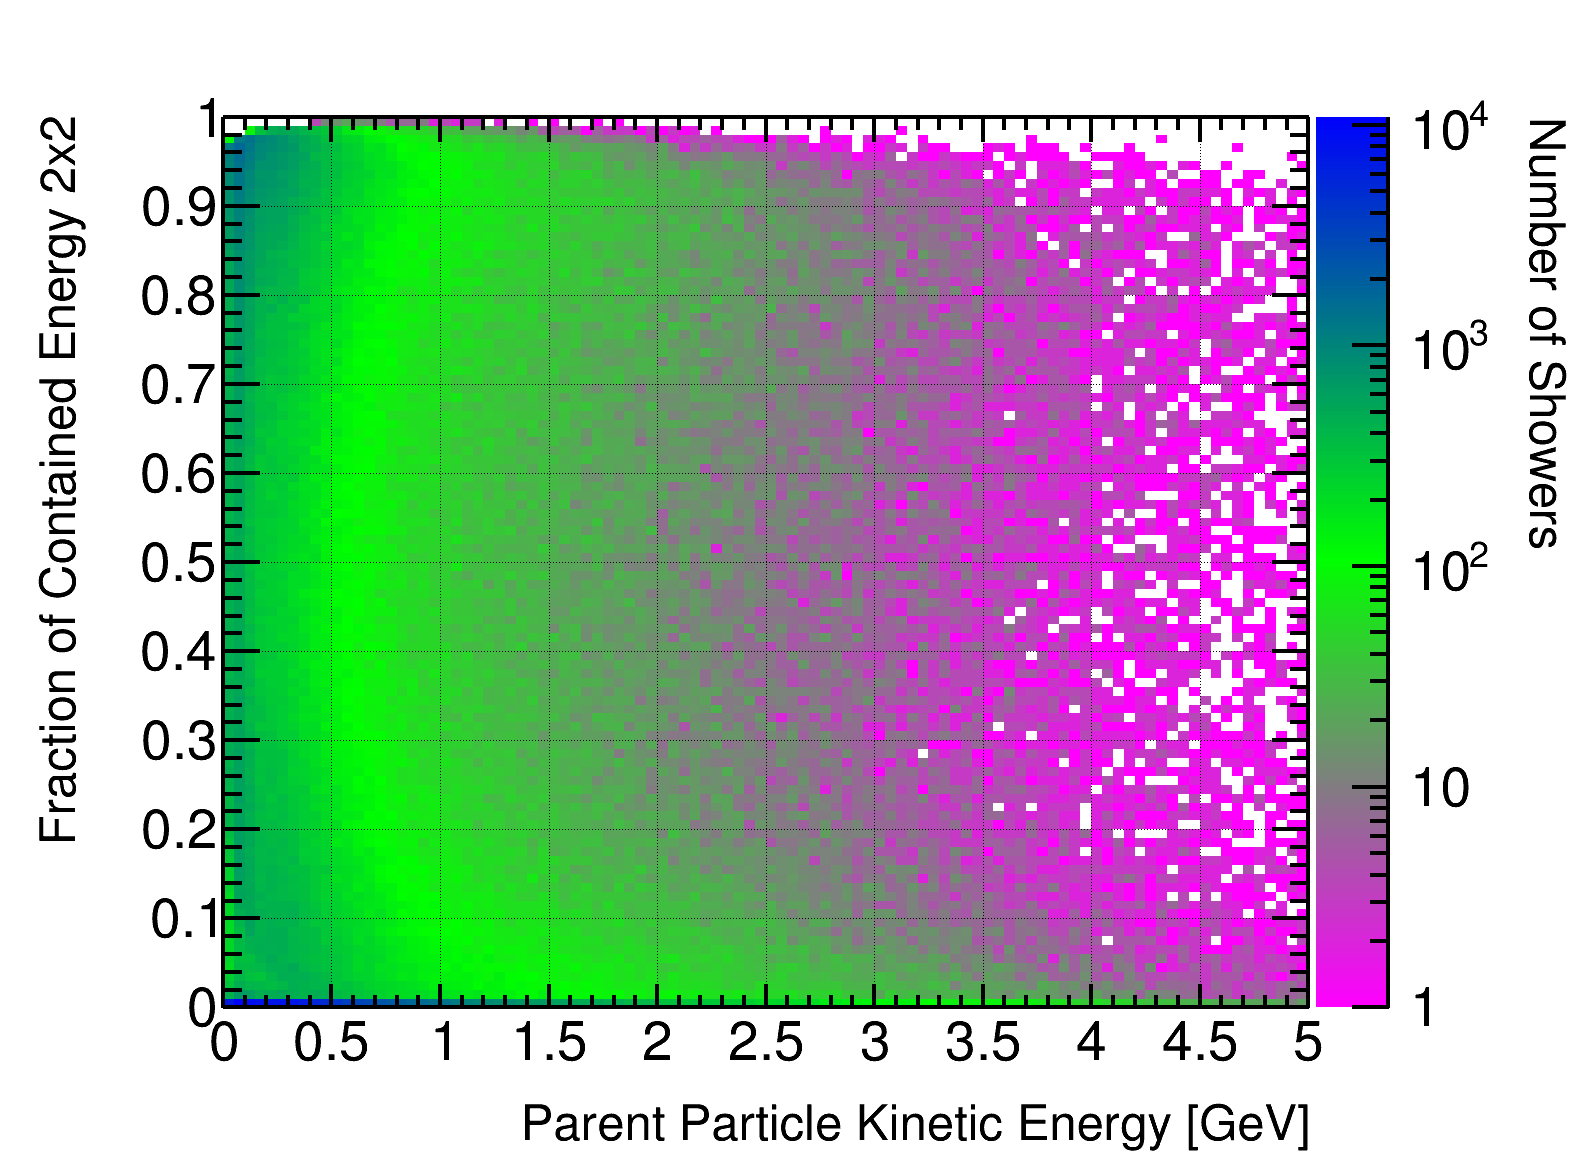
\includegraphics[width=1.0\textwidth]{Pi0_contained_frac_2x2.png}
		\caption{2x2 stand-alone, no fiducialisation.}
		\label{}
	\end{subfigure}	
	\hfill
	\begin{subfigure}[b]{0.49\textwidth}
		\centering
    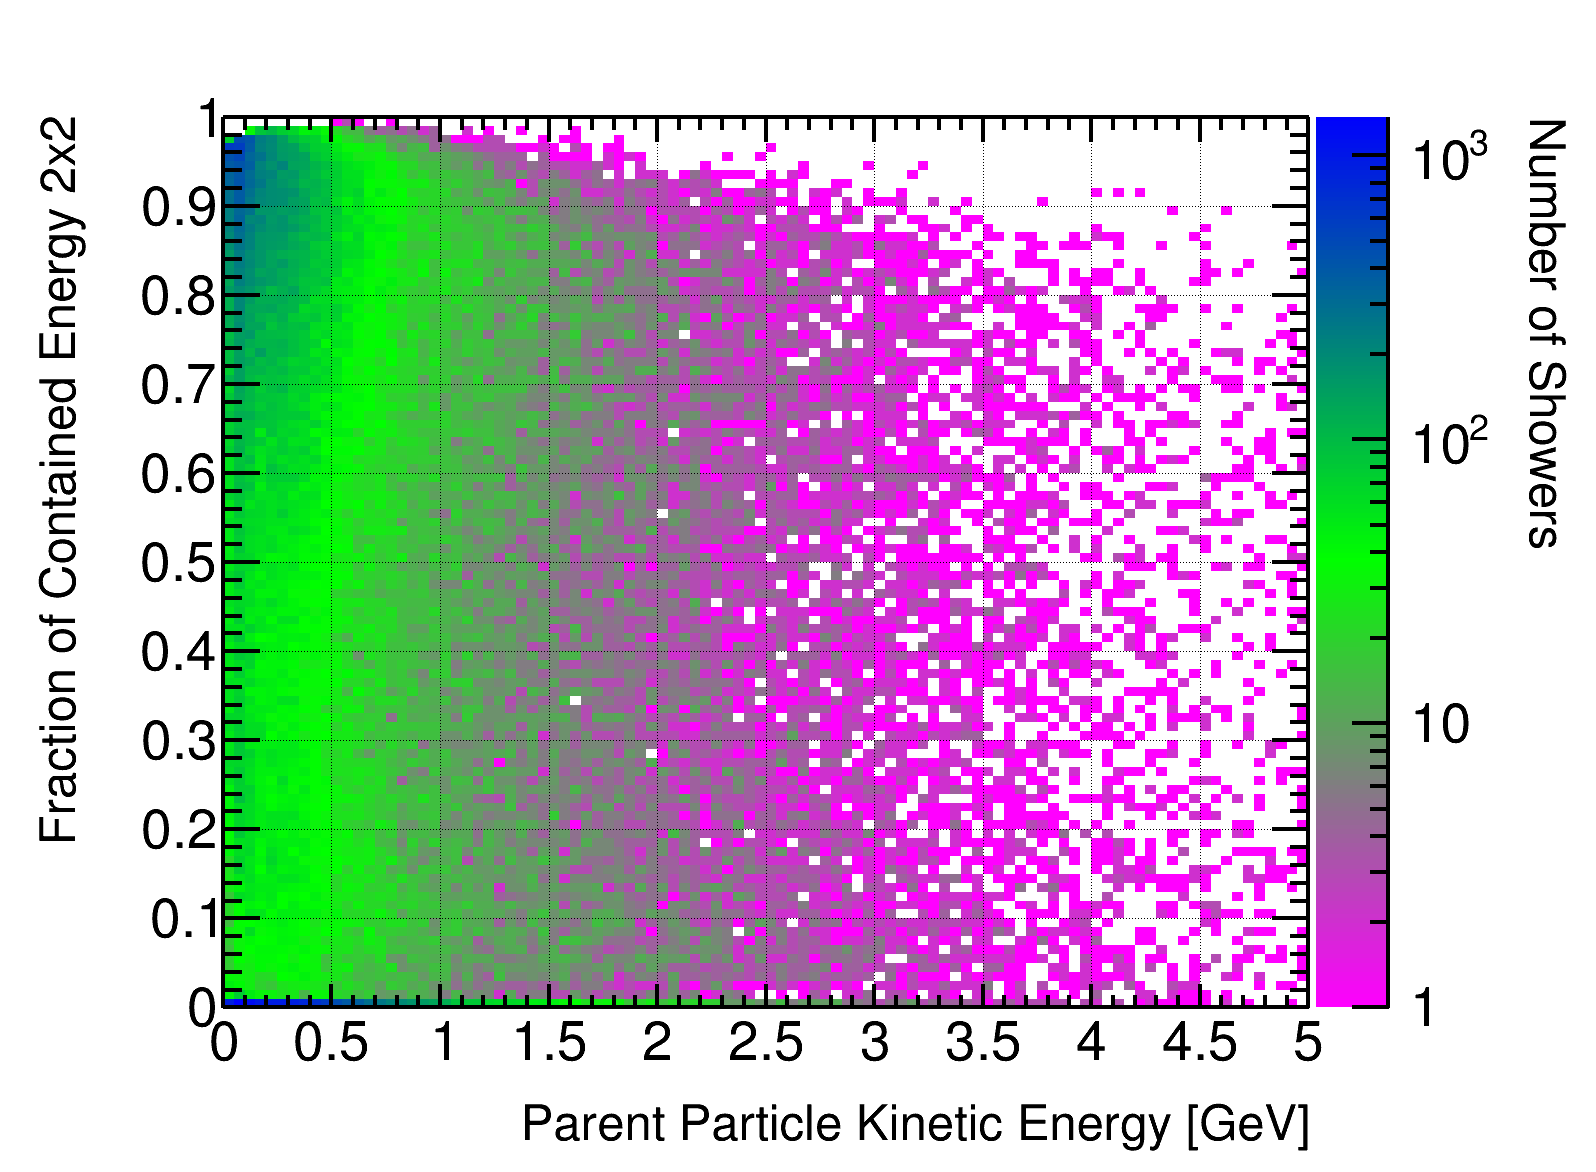
\includegraphics[width=1.0\textwidth]{Pi0_contained_frac_2x2_fiducial.png}
		\caption{2x2 stand-alone, vertex in fiducial volume.}
		\label{}
	\end{subfigure}	
	\begin{subfigure}[b]{0.49\textwidth}
		\centering
		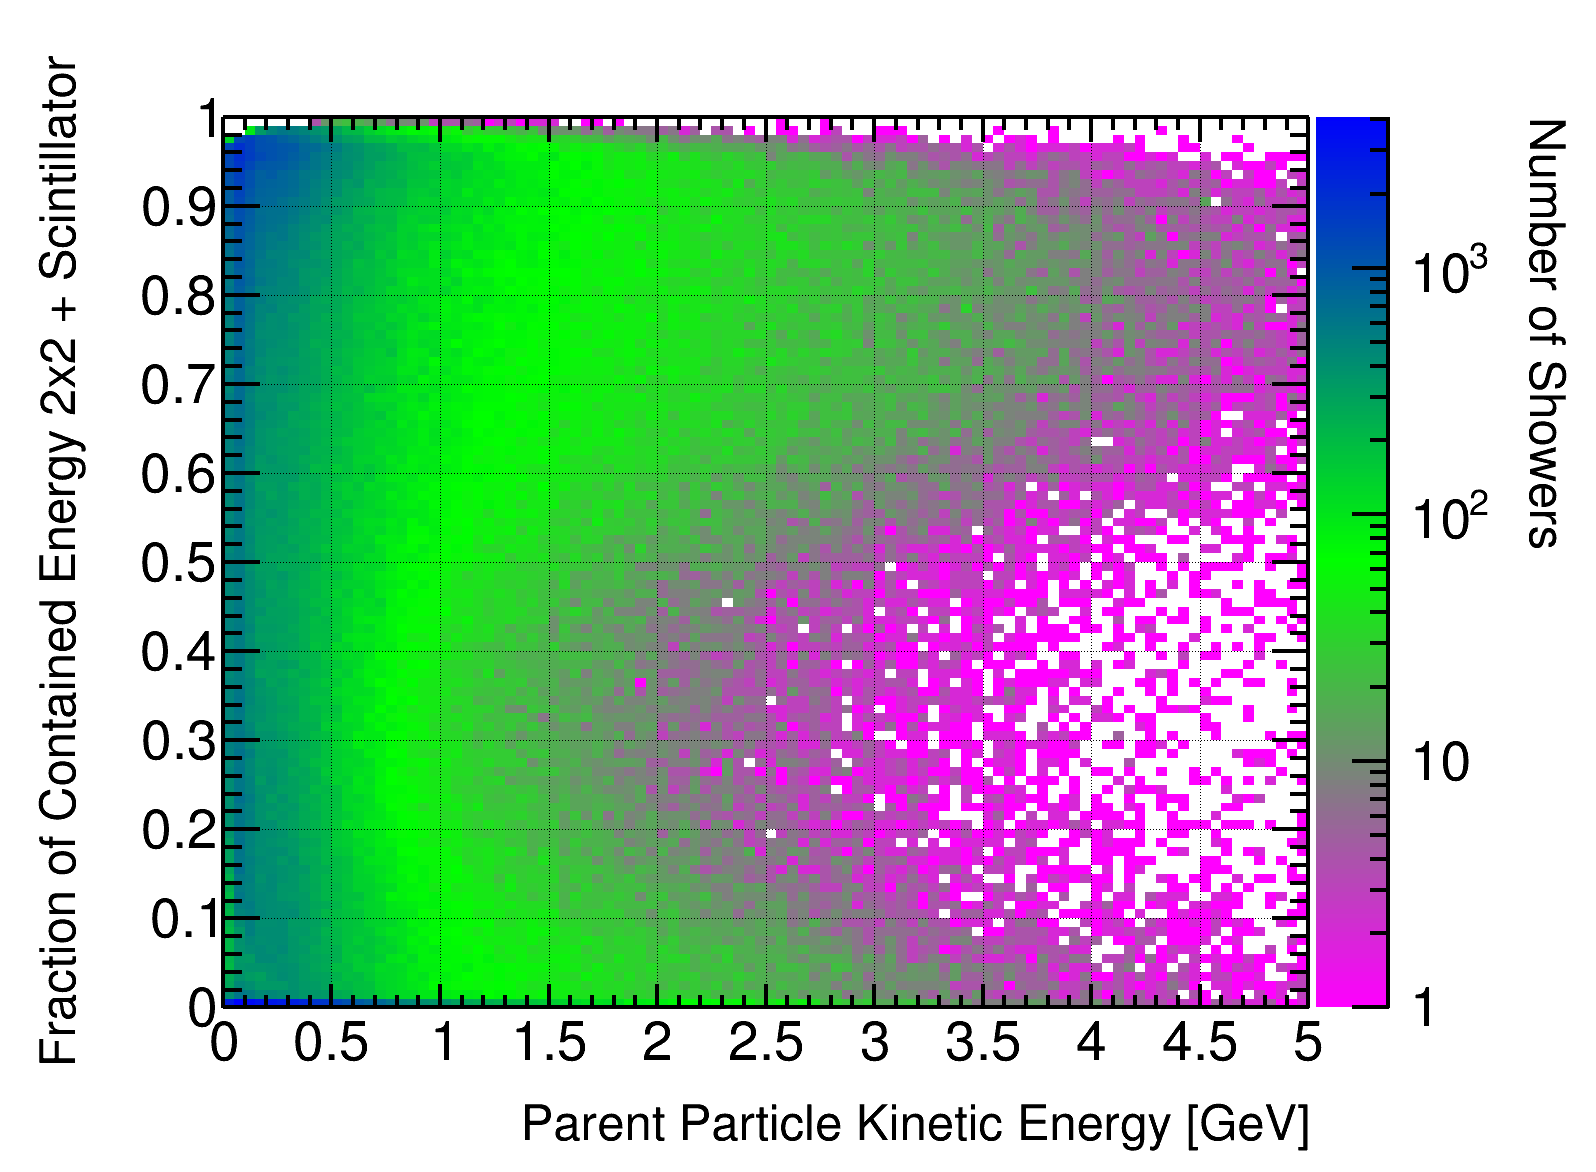
\includegraphics[width=1.0\textwidth]{Pi0_contained_frac_2x2_Scintillator_gap.png}
		\caption{2x2 + tracker, no fiducialisation.}
		\label{}
	\end{subfigure}	
	\hfill
	\begin{subfigure}[b]{0.49\textwidth}
		\centering
		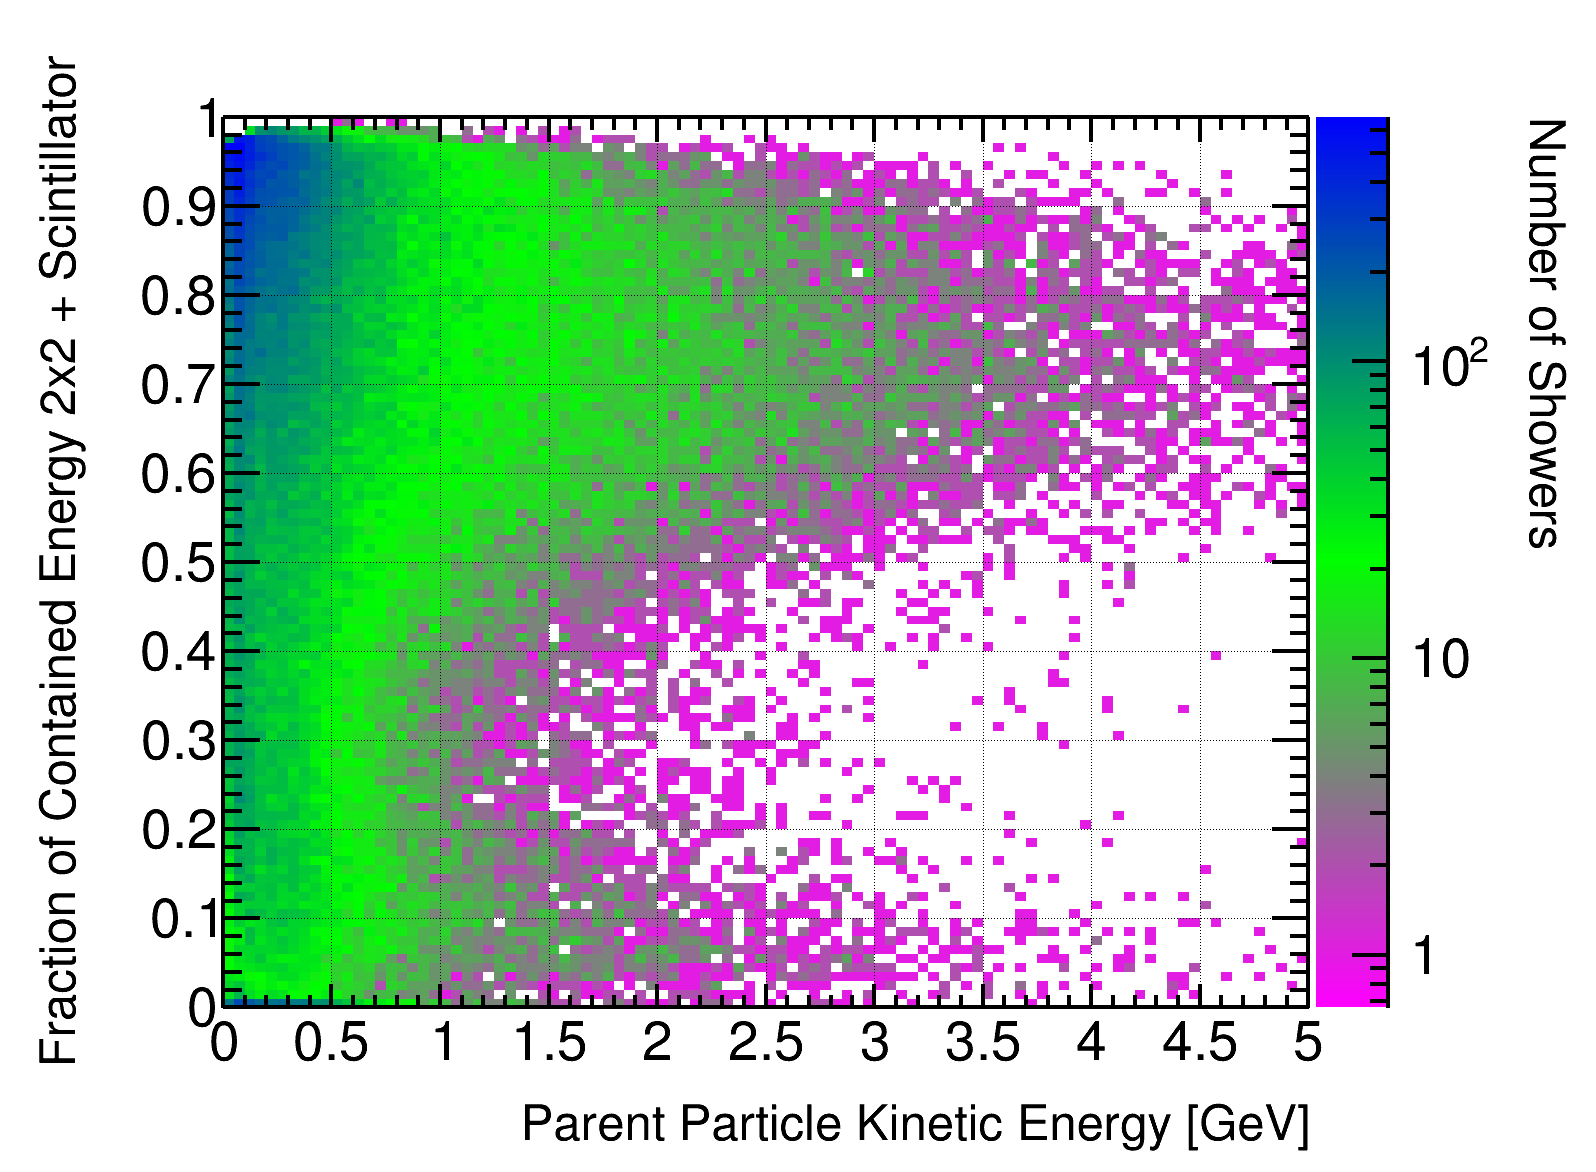
\includegraphics[width=1.0\textwidth]{Pi0_contained_frac_2x2_Scintillator_fiducial_gap.png}
		\caption{2x2 + tracker, vertex in fiducial volume.}
		\label{}
	\end{subfigure}
	\begin{subfigure}[b]{0.49\textwidth}
		\centering
		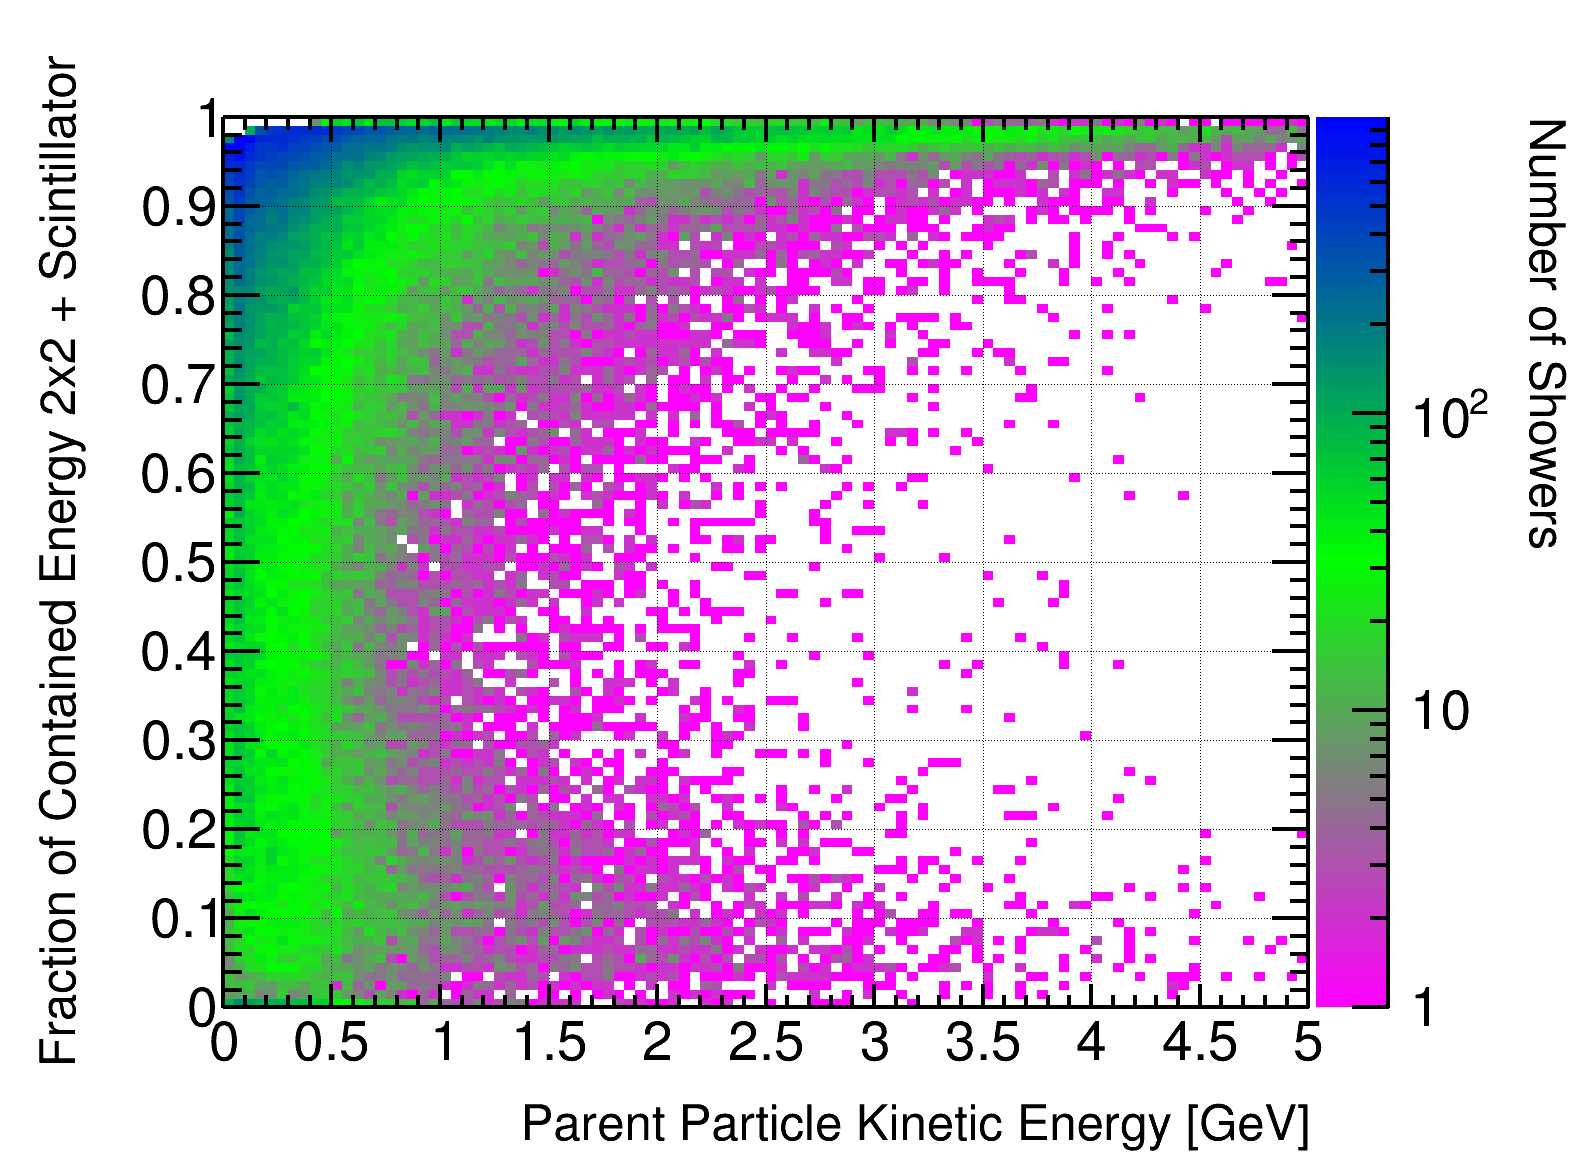
\includegraphics[width=1.0\textwidth]{Pi0_contained_frac_2x2_Scintillator_fiducial.png}
		\caption{2x2 + tracker no gap, vertex in fiducial volume.}
		\label{}
	\end{subfigure}	
  \caption{Fraction of total shower energy (including the $\pi^{0}$~mass) deposited within the active detector volume.}
\end{figure}

\begin{figure}[htbp]
	\centering
	\begin{subfigure}[b]{0.49\textwidth}
		\centering
		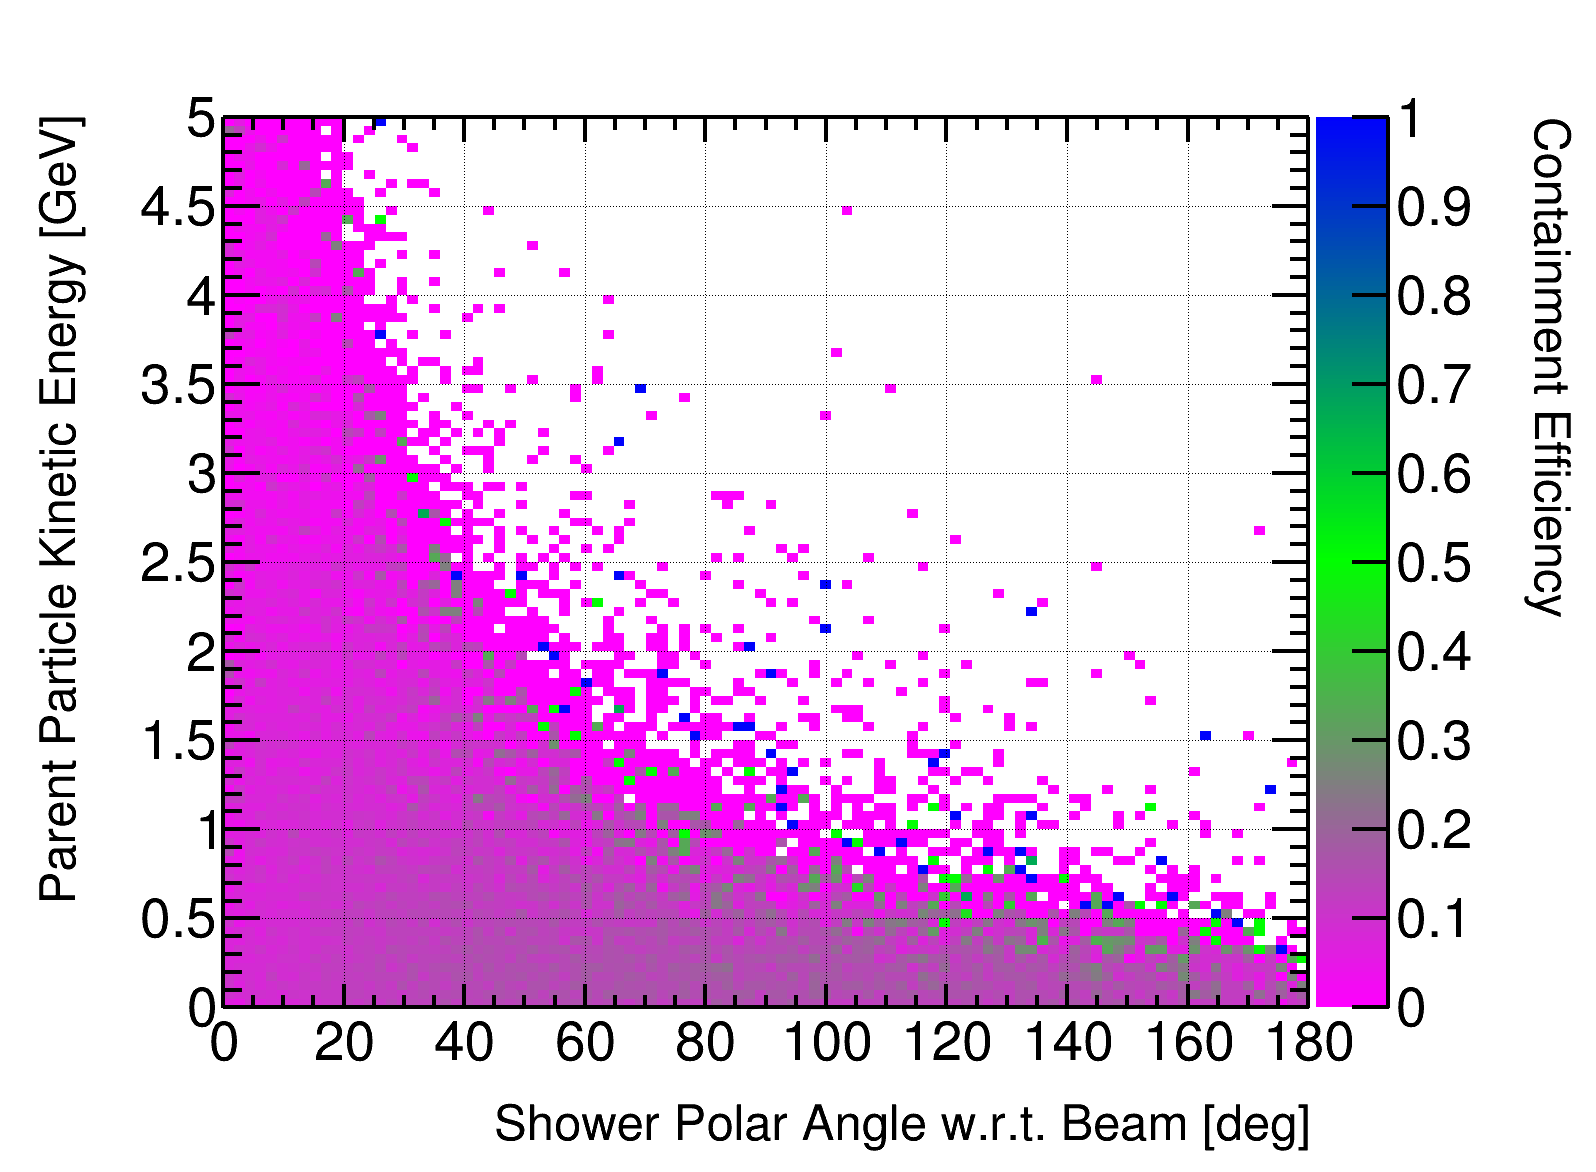
\includegraphics[width=1.0\textwidth]{Pi0_cont_eff_2x2.png}
		\caption{2x2 stand-alone, no fiducialisation.}
		\label{}
	\end{subfigure}	
	\hfill
	\begin{subfigure}[b]{0.49\textwidth}
		\centering
    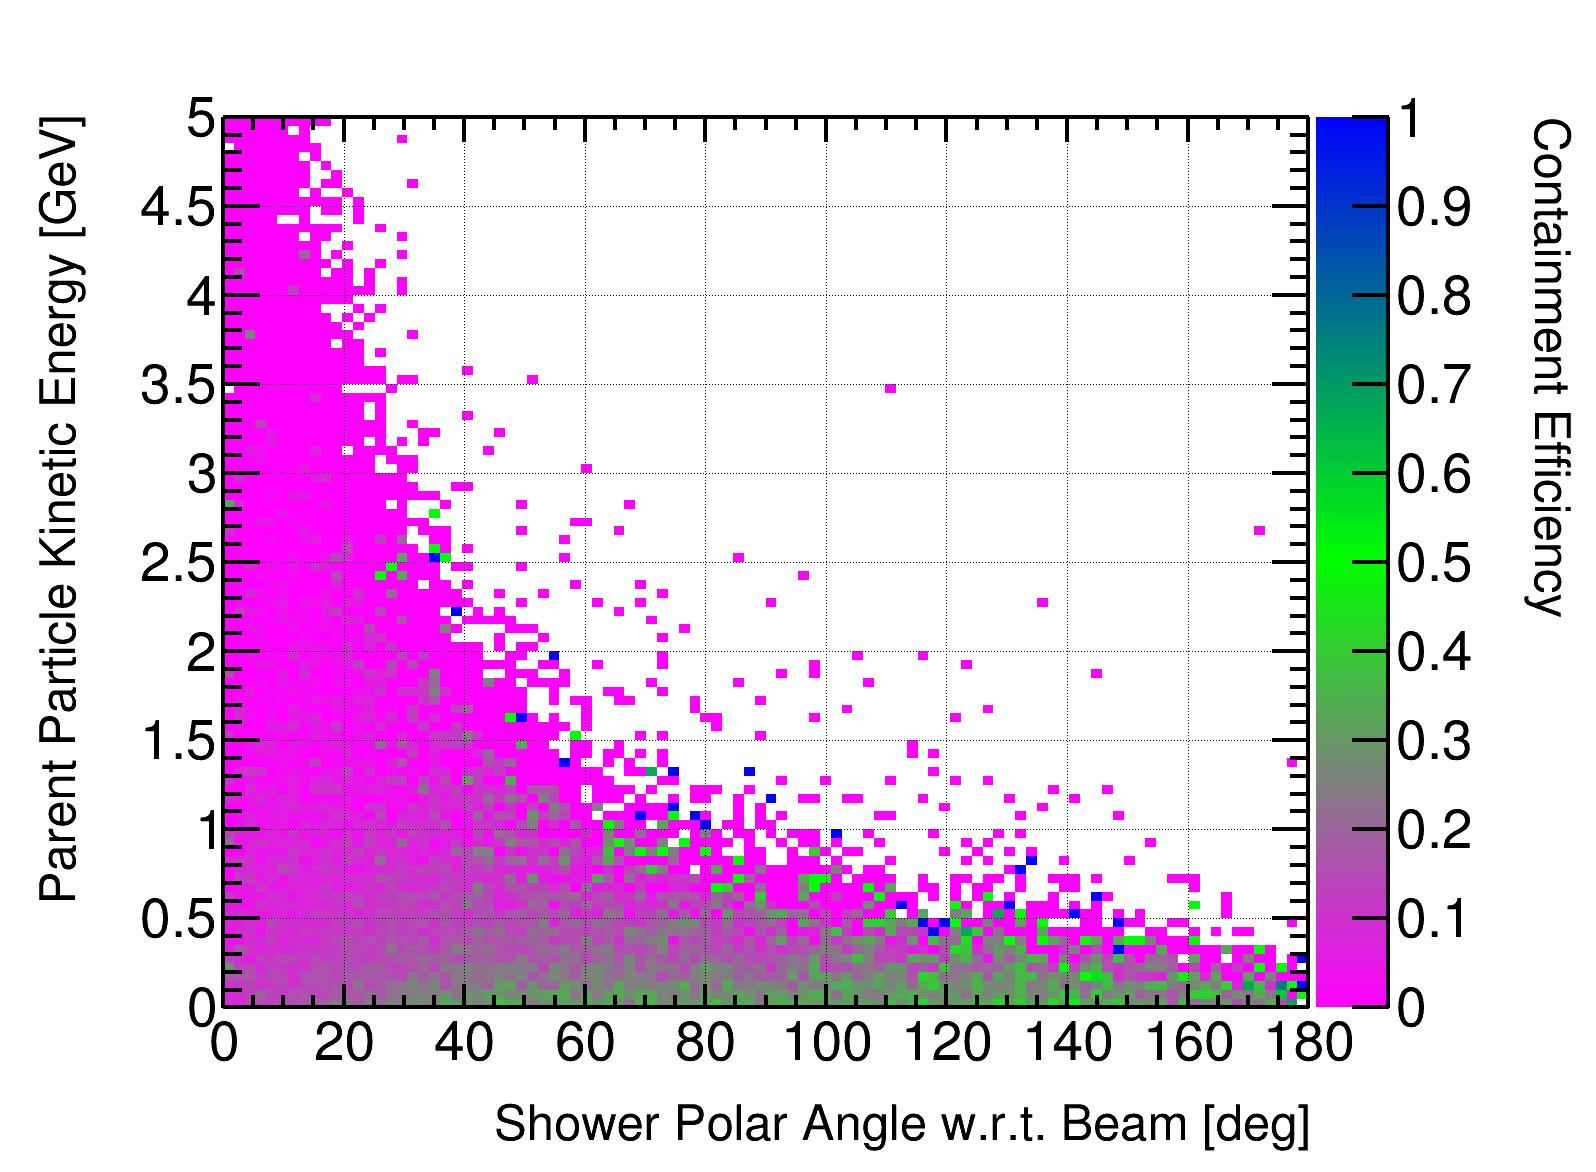
\includegraphics[width=1.0\textwidth]{Pi0_cont_eff_2x2_fiducial.png}
		\caption{2x2 stand-alone, vertex in fiducial volume.}
		\label{}
	\end{subfigure}	
	\begin{subfigure}[b]{0.49\textwidth}
		\centering
		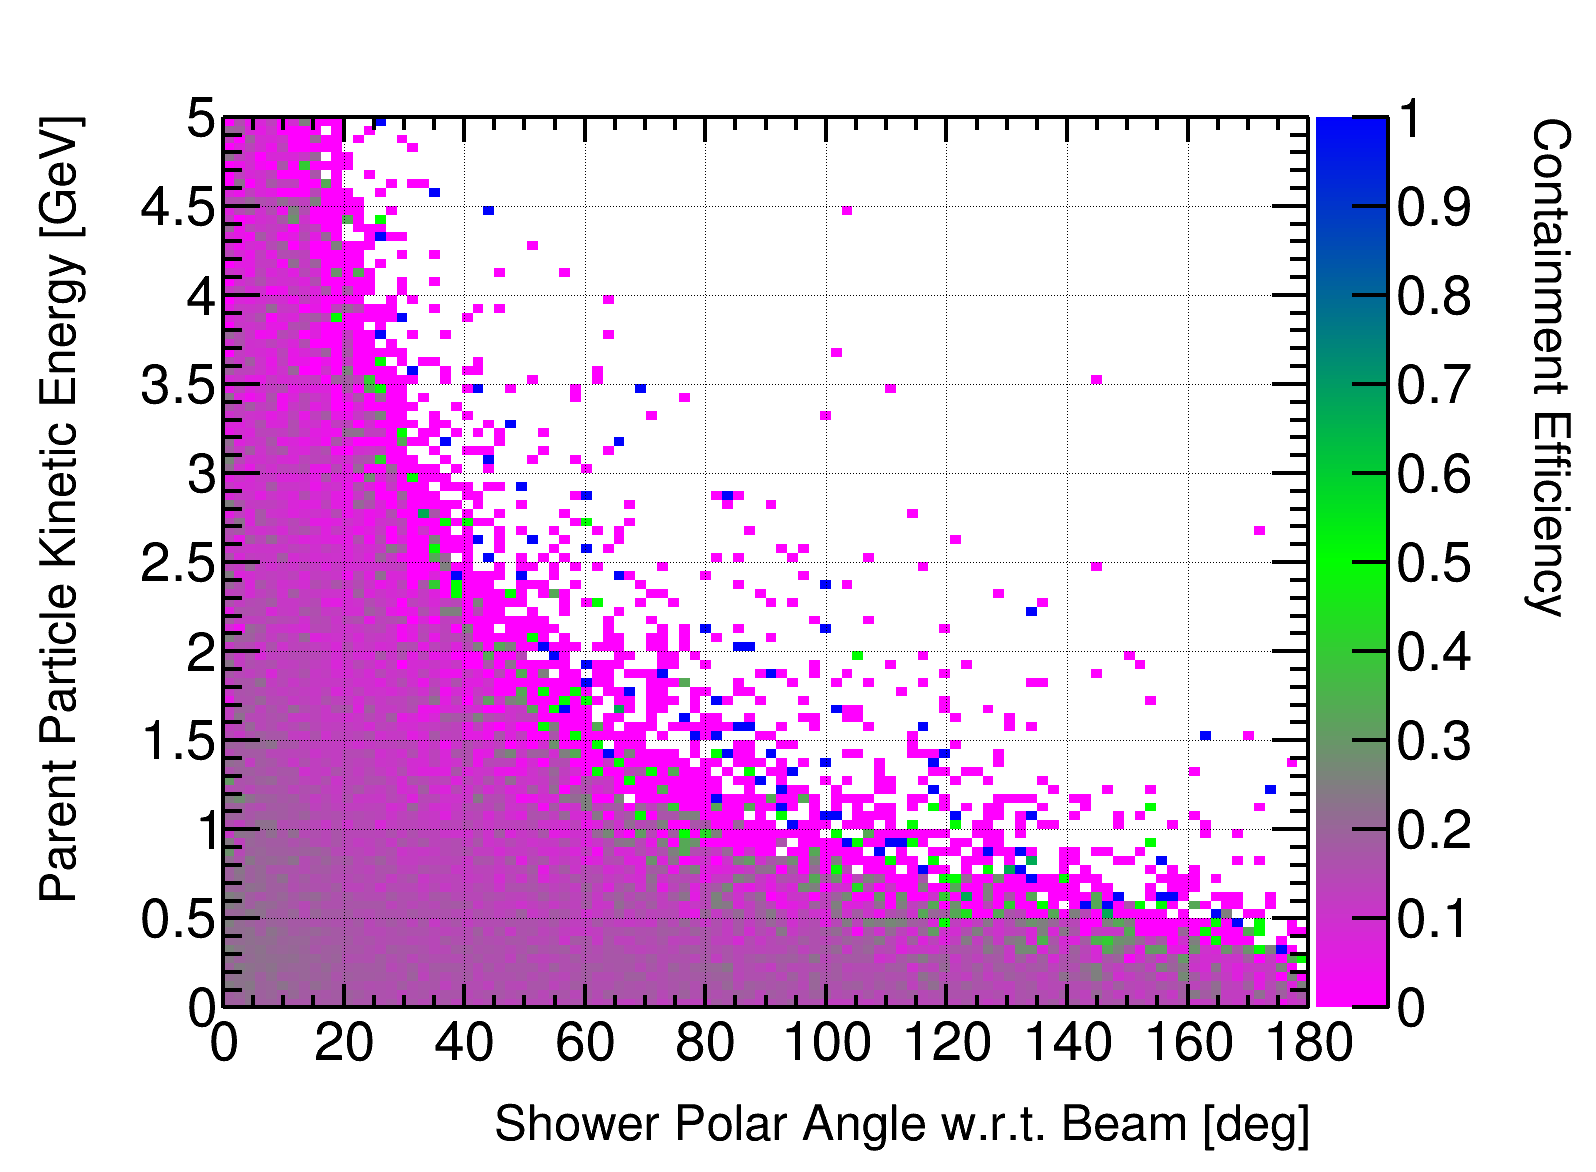
\includegraphics[width=1.0\textwidth]{Pi0_cont_eff_2x2_Scintillator_gap.png}
		\caption{2x2 + tracker, no fiducialisation.}
		\label{}
	\end{subfigure}	
	\hfill
	\begin{subfigure}[b]{0.49\textwidth}
		\centering
		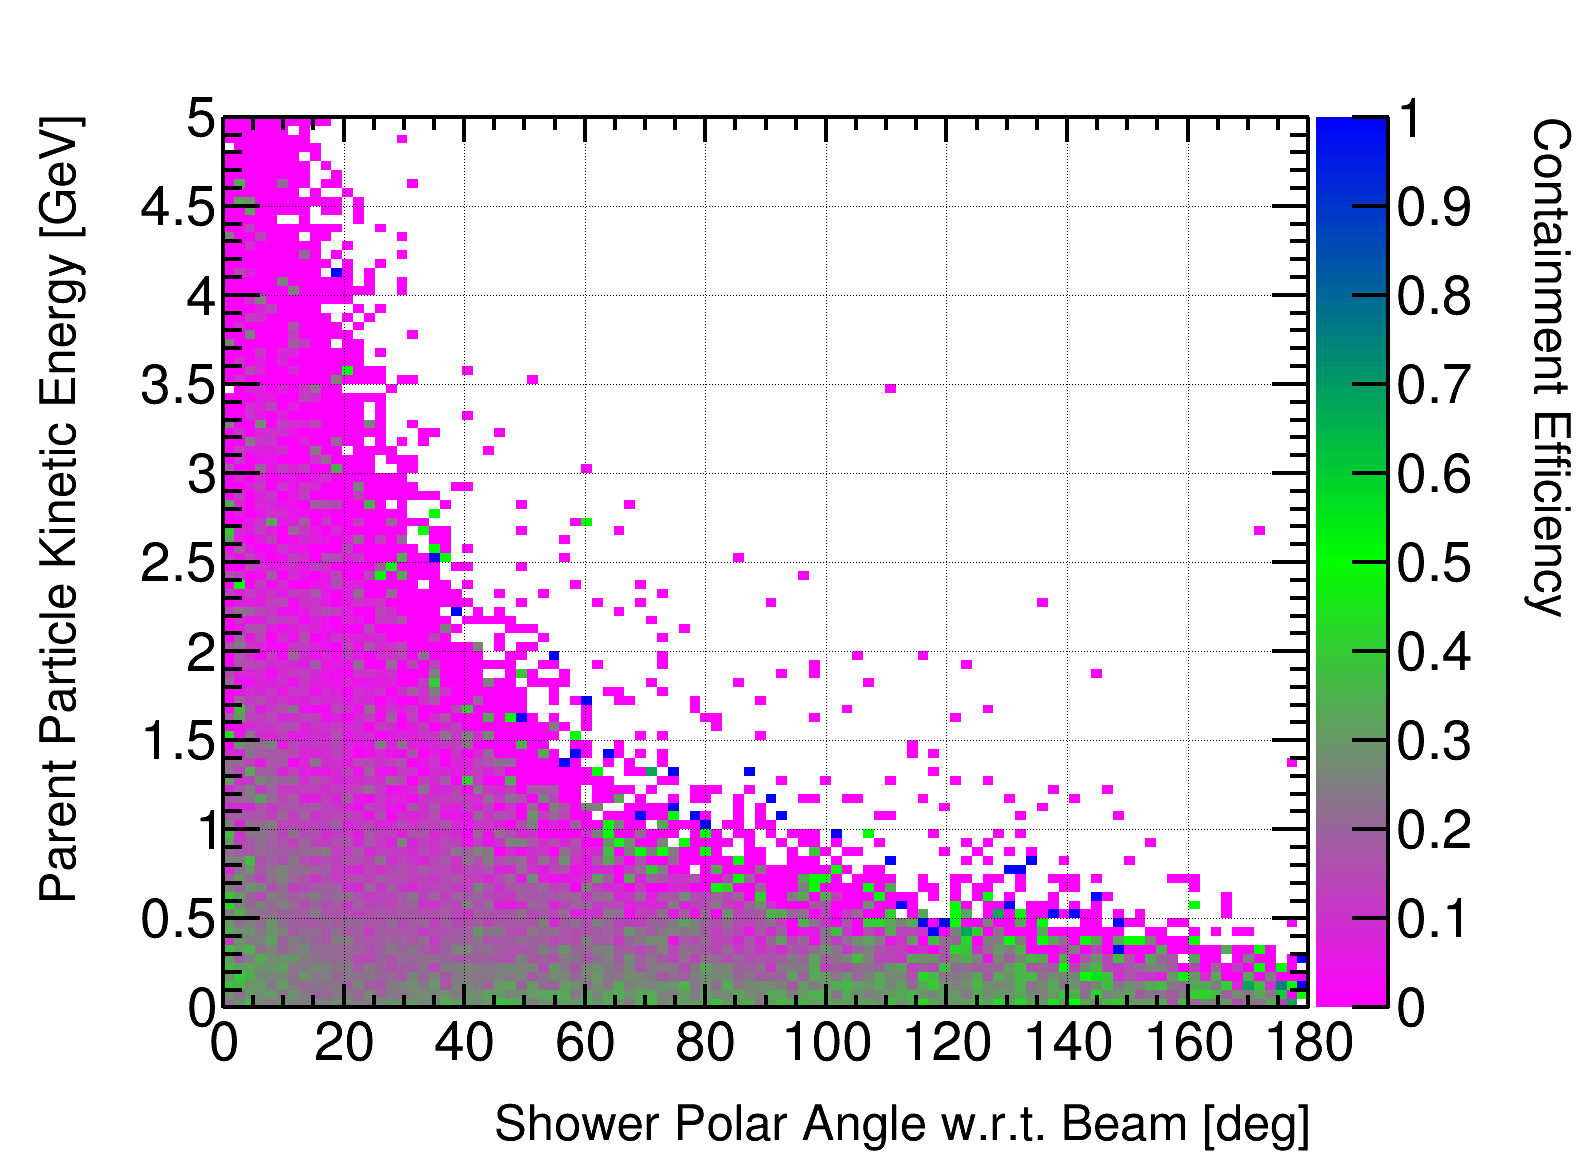
\includegraphics[width=1.0\textwidth]{Pi0_cont_eff_2x2_Scintillator_fiducial_gap.png}
		\caption{2x2 + tracker, vertex in fiducial volume.}
		\label{}
	\end{subfigure}
	\begin{subfigure}[b]{0.49\textwidth}
		\centering
		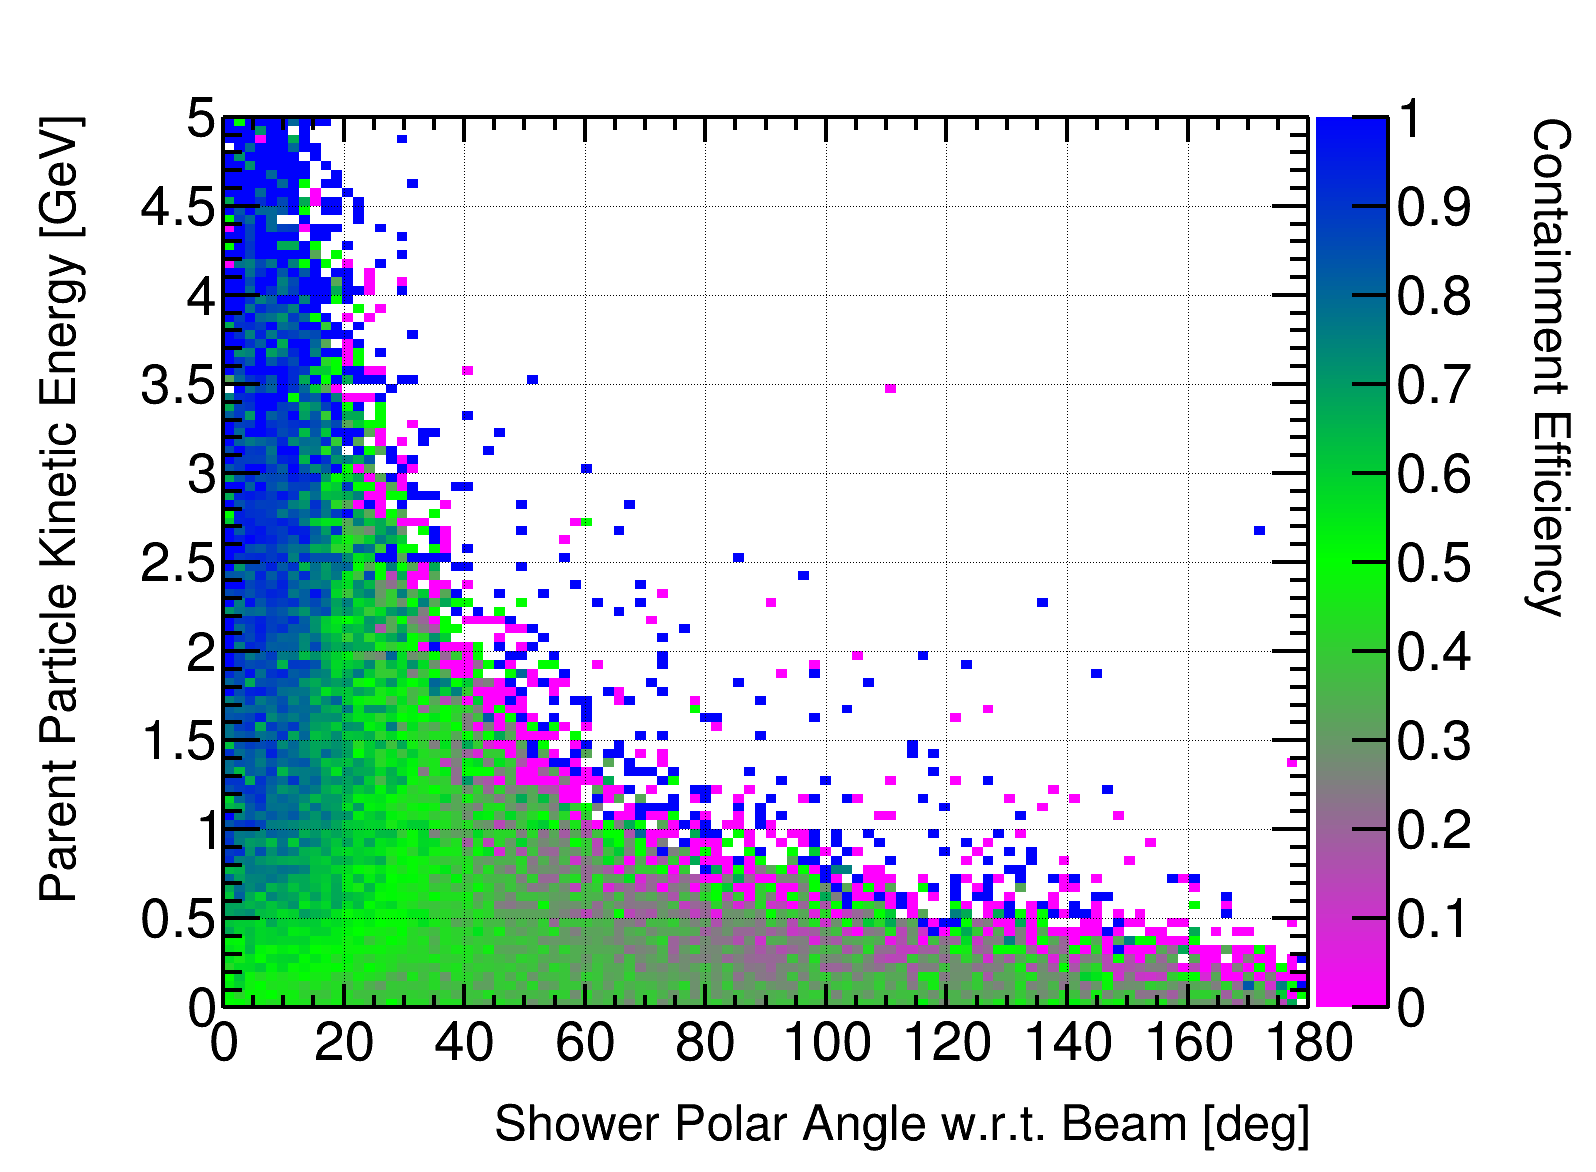
\includegraphics[width=1.0\textwidth]{Pi0_cont_eff_2x2_Scintillator_fiducial.png}
		\caption{2x2 + tracker no gap, vertex in fiducial volume.}
		\label{}
	\end{subfigure}	
  \caption{Shower-containment efficiency. A shower is classed as contained if at least 90\% of the total shower energy (including the $\pi^{0}$~mass) is deposited within the active detector volume.}
\end{figure}

\subsubsection{Proton Induced Showers}
\begin{figure}[htbp]
	\centering
	\begin{subfigure}[b]{0.49\textwidth}
		\centering
		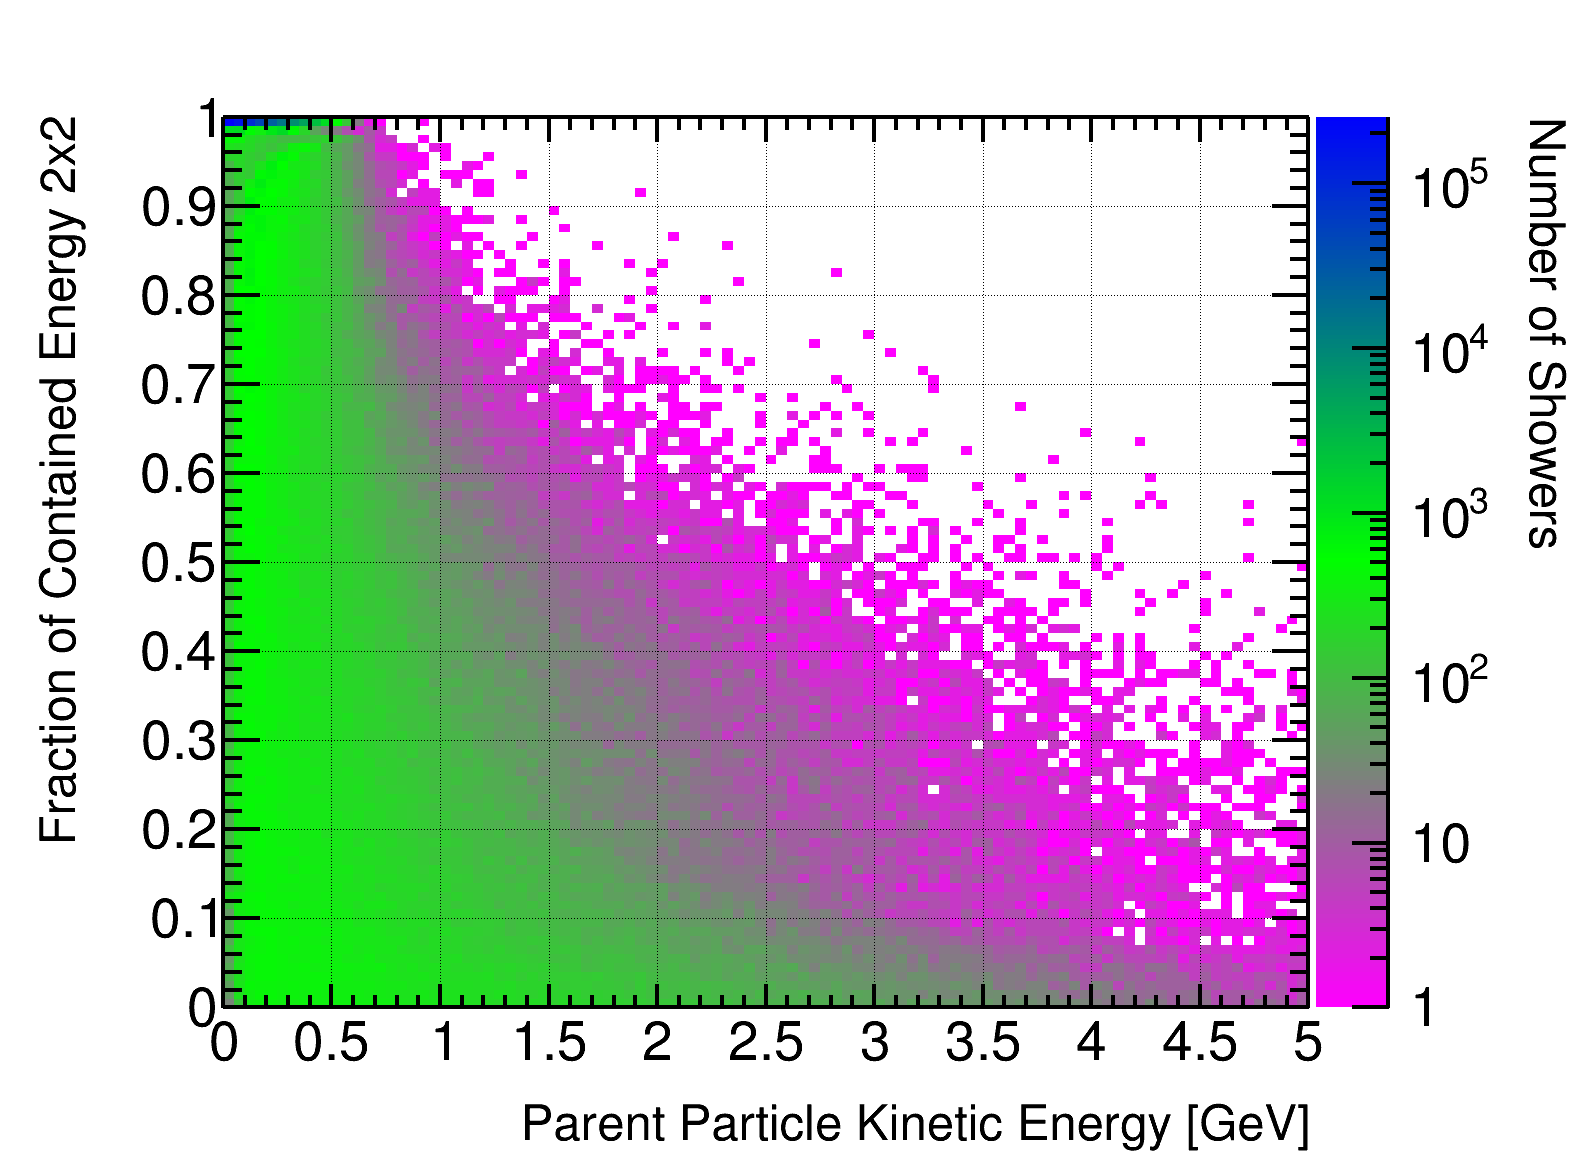
\includegraphics[width=1.0\textwidth]{P_contained_frac_2x2.png}
		\caption{2x2 stand-alone, no fiducialisation.}
		\label{}
	\end{subfigure}	
	\hfill
	\begin{subfigure}[b]{0.49\textwidth}
		\centering
		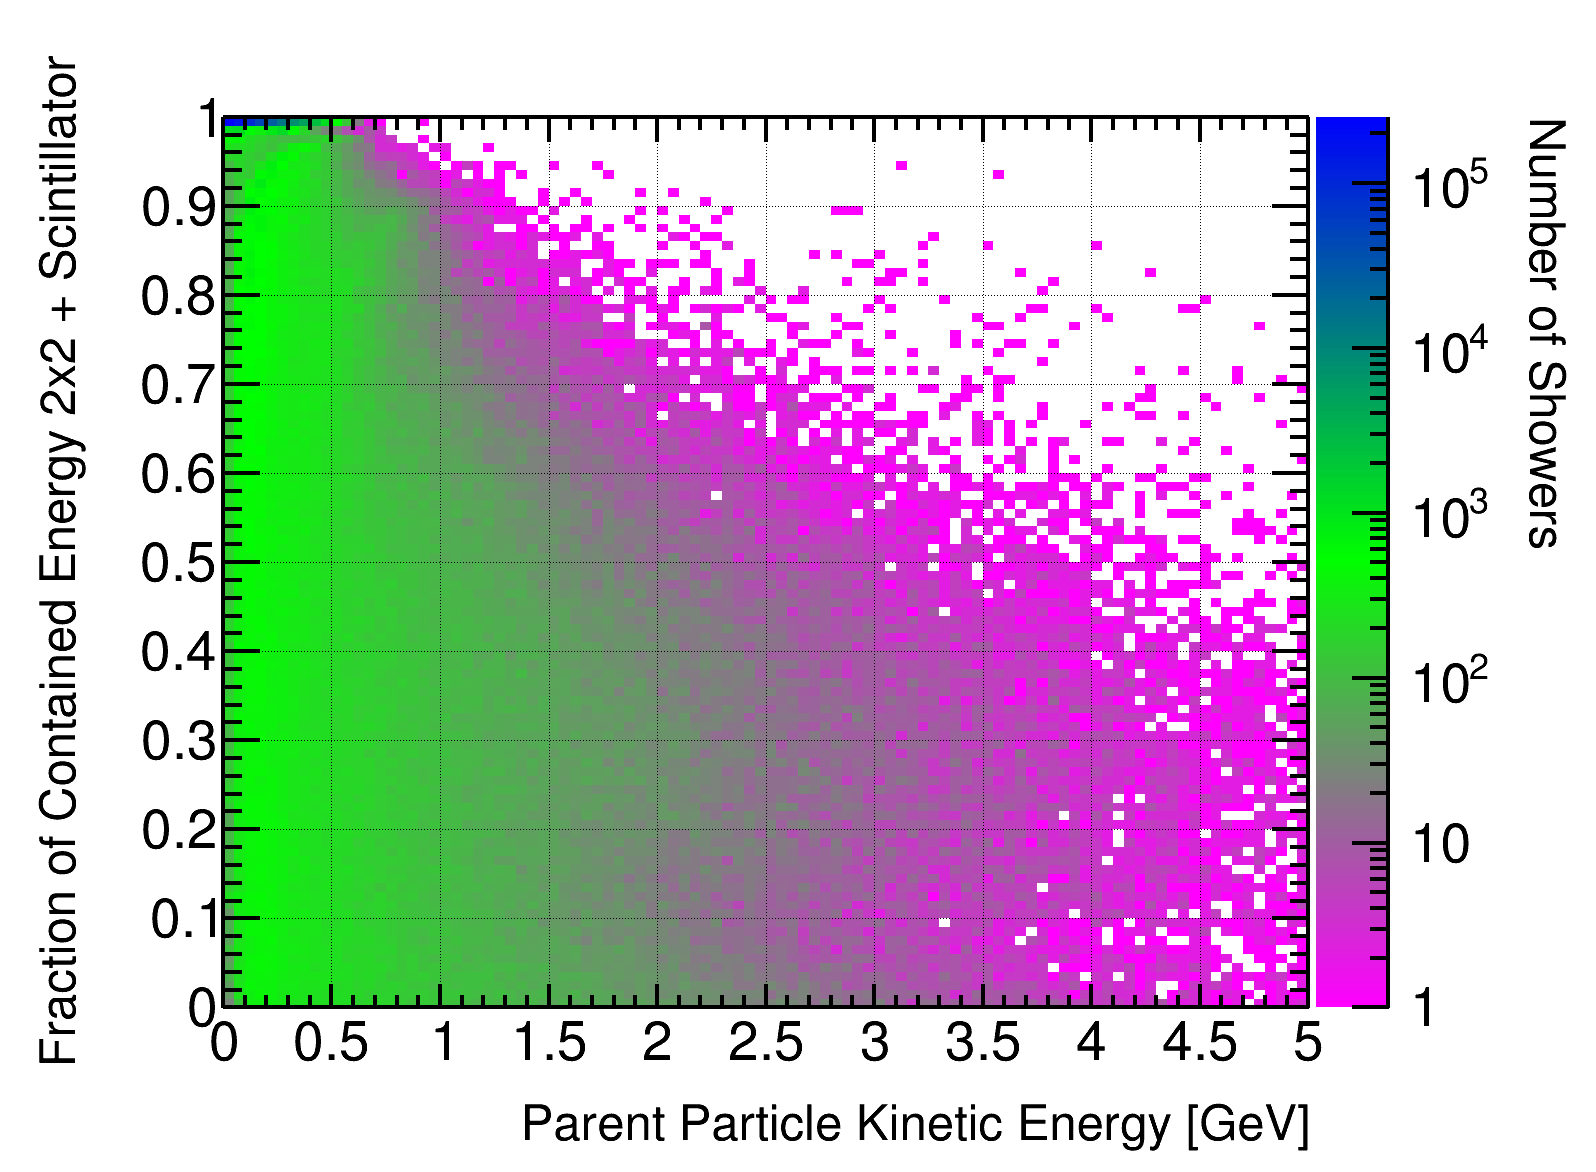
\includegraphics[width=1.0\textwidth]{P_contained_frac_2x2_Scintillator_gap.png}
		\caption{2x2 + tracker, no fiducialisation.}
		\label{}
	\end{subfigure}	
	\caption{Fraction of initial proton kinetic energy deposited within the active detector volume.}
\end{figure}

\begin{figure}[htbp]
	\centering
	\begin{subfigure}[b]{0.49\textwidth}
		\centering
		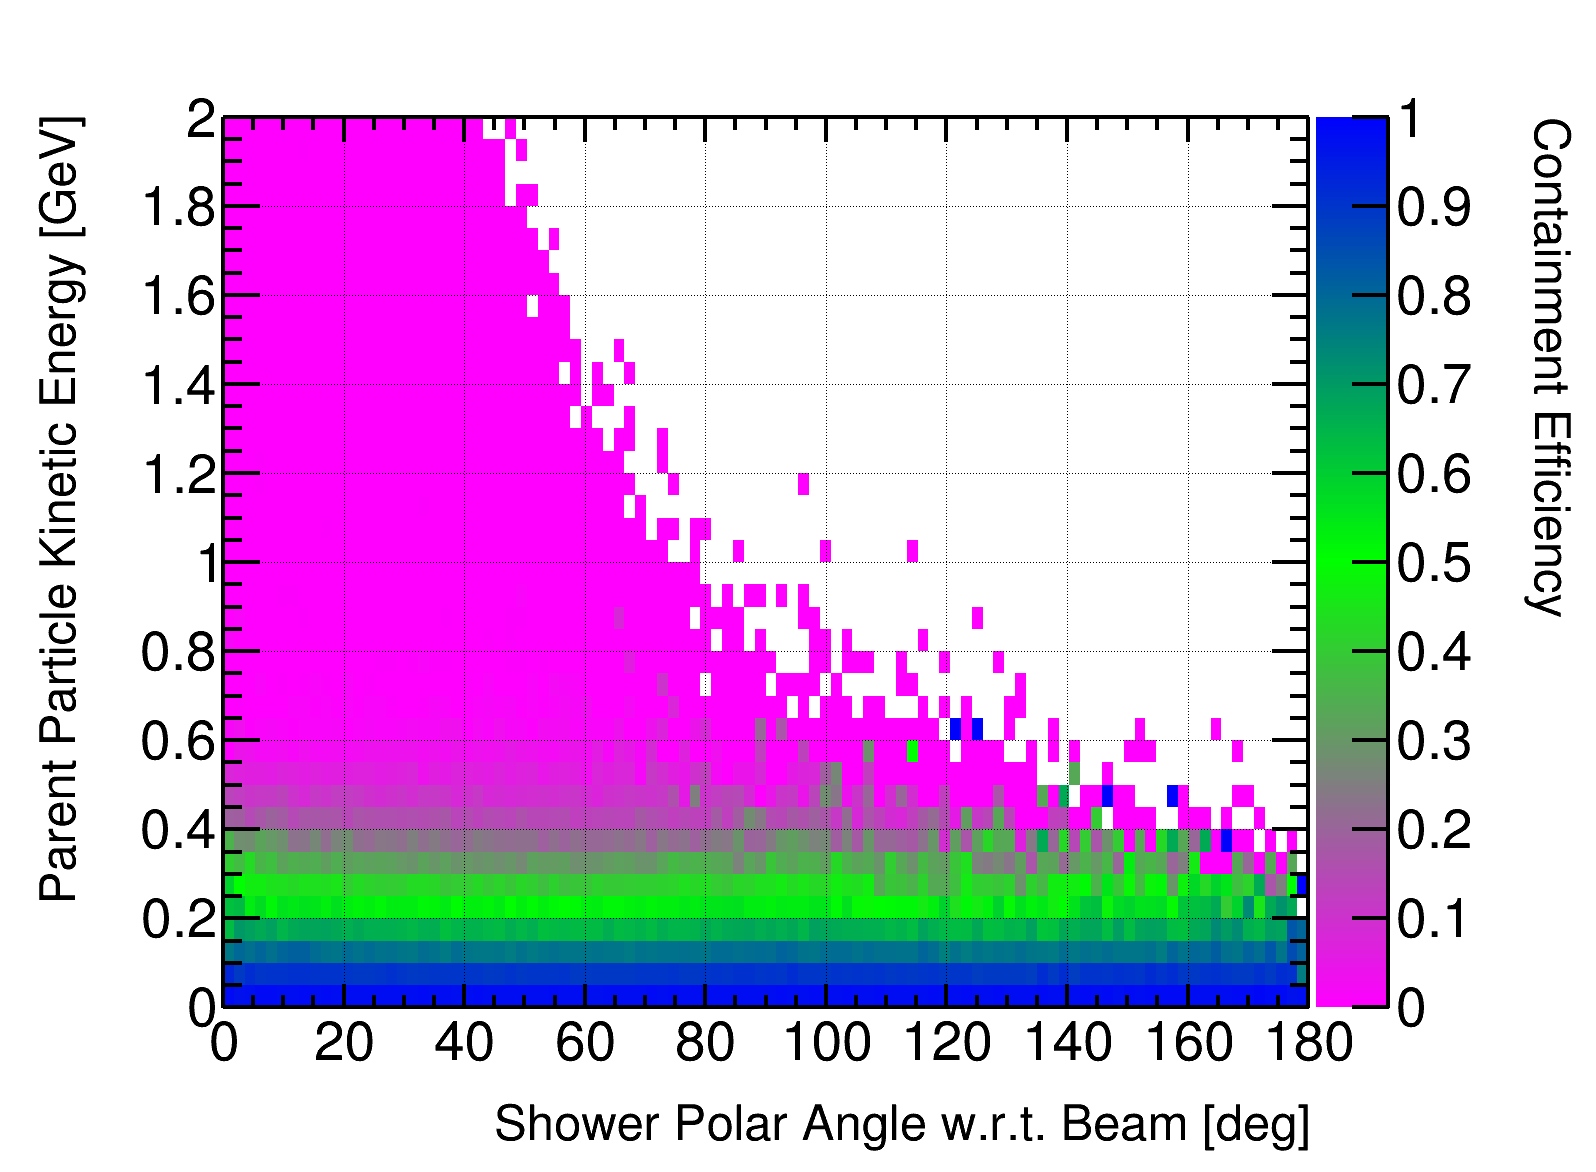
\includegraphics[width=1.0\textwidth]{P_cont_eff_2x2.png}
		\caption{2x2 stand-alone, no fiducialisation.}
		\label{}
	\end{subfigure}	
	\hfill
	\begin{subfigure}[b]{0.49\textwidth}
		\centering
		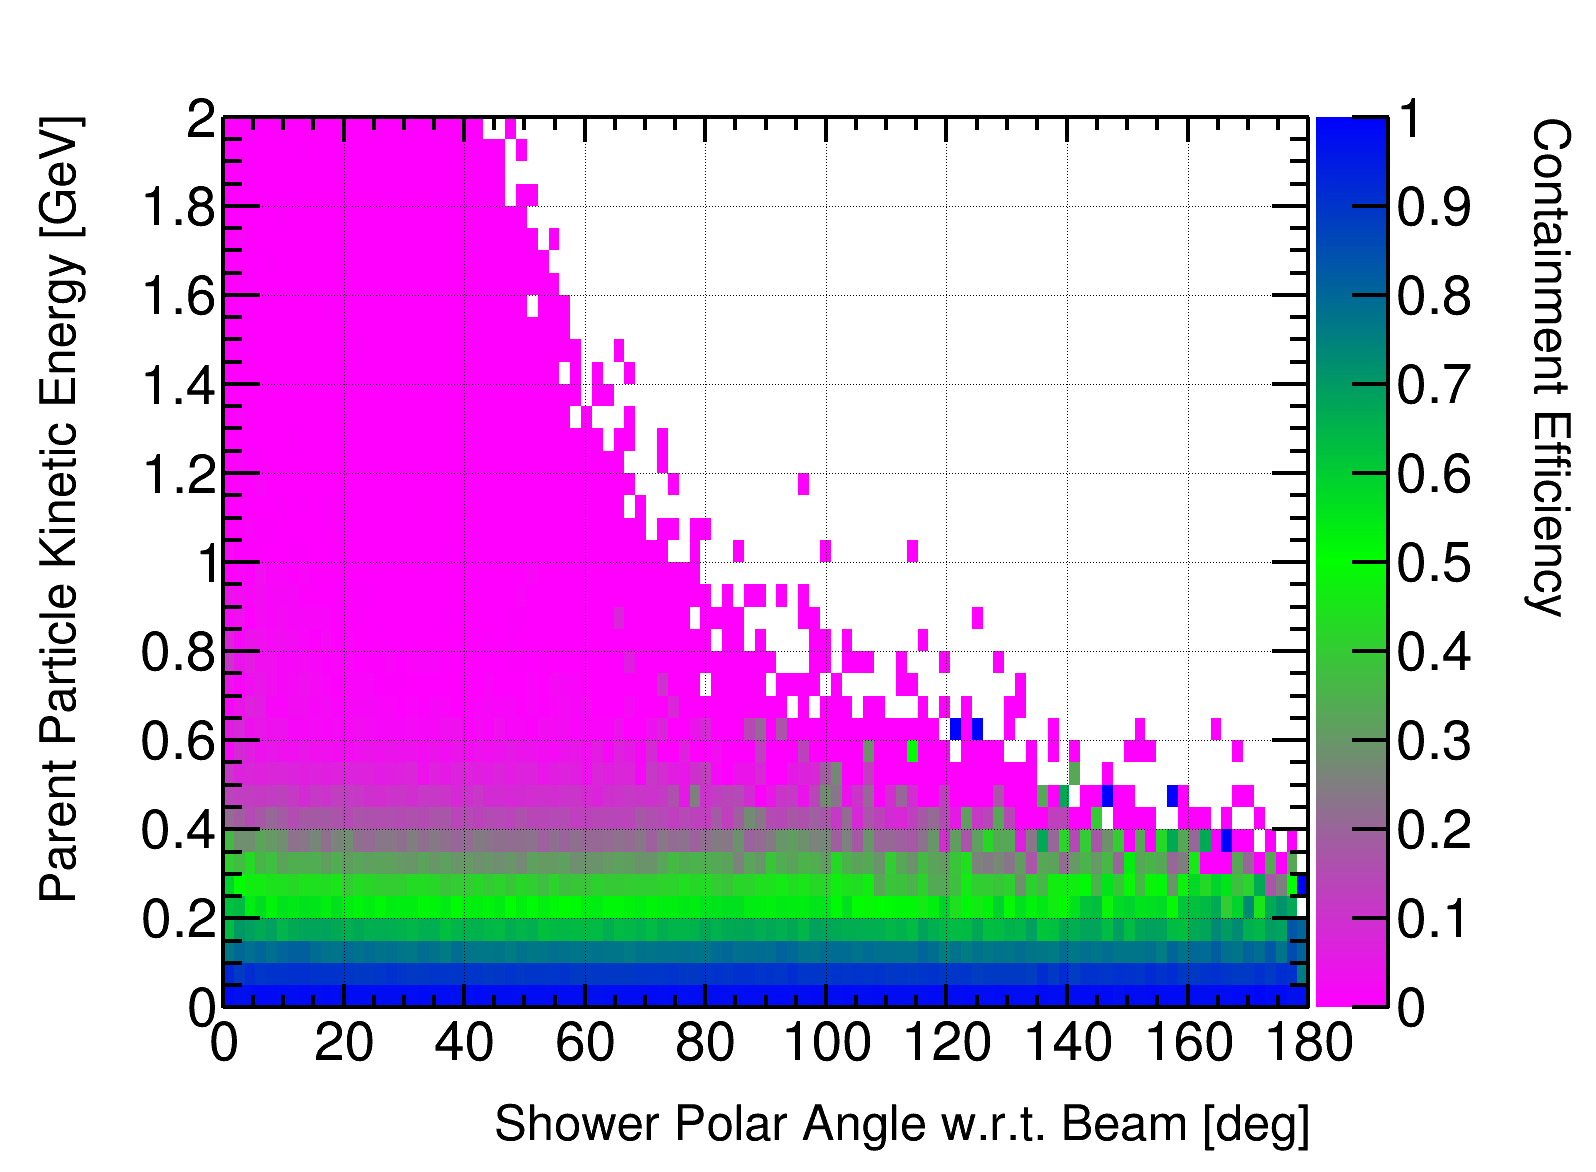
\includegraphics[width=1.0\textwidth]{P_cont_eff_2x2_Scintillator_gap.png}
		\caption{2x2 + tracker, no fiducialisation.}
		\label{}
	\end{subfigure}	
	\caption{Shower-containment efficiency. A shower is classed as contained if at least 90\% of the initial proton kinetic energy is deposited within the active detector volume.}
\end{figure}

%%%%%%%%%%%%%%%%%%%%%%%%%%%%%%%%%%%%%%%%%%%%%%%%%%%%%%%%%%%%%%%%%%%%%%%%%%%%%%%
%---References---
%%%%%%%%%%%%%%%%%%%%%%%%%%%%%%%%%%%%%%%%%%%%%%%%%%%%%%%%%%%%%%%%%%%%%%%%%%%%%%%
%\begin{thebibliography}{99}
%\begin{small}

%\bibitem{Abi:2018dnh} 
  %B.~Abi {\it et al.} [DUNE Collaboration],
  %``The DUNE Far Detector Interim Design Report Volume 1: Physics, Technology and Strategies,''
  %arXiv:1807.10334 [physics.ins-det].
  %%CITATION = ARXIV:1807.10334;%%
  %1 citations counted in INSPIRE as of 24 Aug 2018
  
%\end{small}
%\end{thebibliography}

%%%%%%%%%%%%%%%%%%%%%%%%%%%%%%%%%%%%%%%%%%%%%%%%%%%%%%%%%%%%%%%%%%%%%%%%%%%%%%%
%---Appendix: First Appendix---
%%%%%%%%%%%%%%%%%%%%%%%%%%%%%%%%%%%%%%%%%%%%%%%%%%%%%%%%%%%%%%%%%%%%%%%%%%%%%%%
%\appendix
%\section{First Appendix}

\end{document}
